\section{Numerical Results and Comparisons}\label{sec:results}


The solutions to the PNP problem exhibit a specific behavior that was 
described above. In order to find the best adaptive method to deal with 
this type of problems, we performed numerous computations using all 
adaptivity modes in both the single-mesh and multi-mesh regimes.
In the numerical experiments we paid attention to the 
relative error, cumulative CPU time, and problem size 
in terms of number of degrees of freedom (DOF) in each 
time step. The scaled variables $c$
and $\varphi$ and the unscaled time $t$ are used to present the solutions.
The simulations were performed with physical time step of $0.05$~s and
the final time of $3.0$~s was chosen as it is close to the time
scaling constant~$\tau$.

We used two types of initial meshes --- a finer mesh shown 
in Fig.~\ref{fig:mesh}~(b) was used for \emph{p}-adaptivity
and a very coarse initial mesh shown in  Fig.~\ref{fig:mesh}~(a) was 
used for $h$-adaptivity and $hp$-adaptivity.

\begin{figure}[!ht]
  \begin{centering}
  
\includegraphics[width=.9\columnwidth]{mesh}
  \caption{\label{fig:mesh} Initial coarse mesh (a),
  	refined mesh (b), and symmetrically refined mesh for length scale study (c). 
	The coarse mesh (a)
	and refined mesh (b) were used in the initial calculations, the latter one
	in case of \emph{p}-adaptivity (including HP\_ANISO\_P).}
  \end{centering}
\end{figure}

An example of the solution at $t=0.1\ s$ and $t=3.0\ s$ 
calculated with the HP\_ANISO refinement mode is shown
in Figs.~\ref{fig:cphi-1}~and~\ref{fig:cphi-2}. 

\begin{figure}[!ht]
  \begin{centering}
  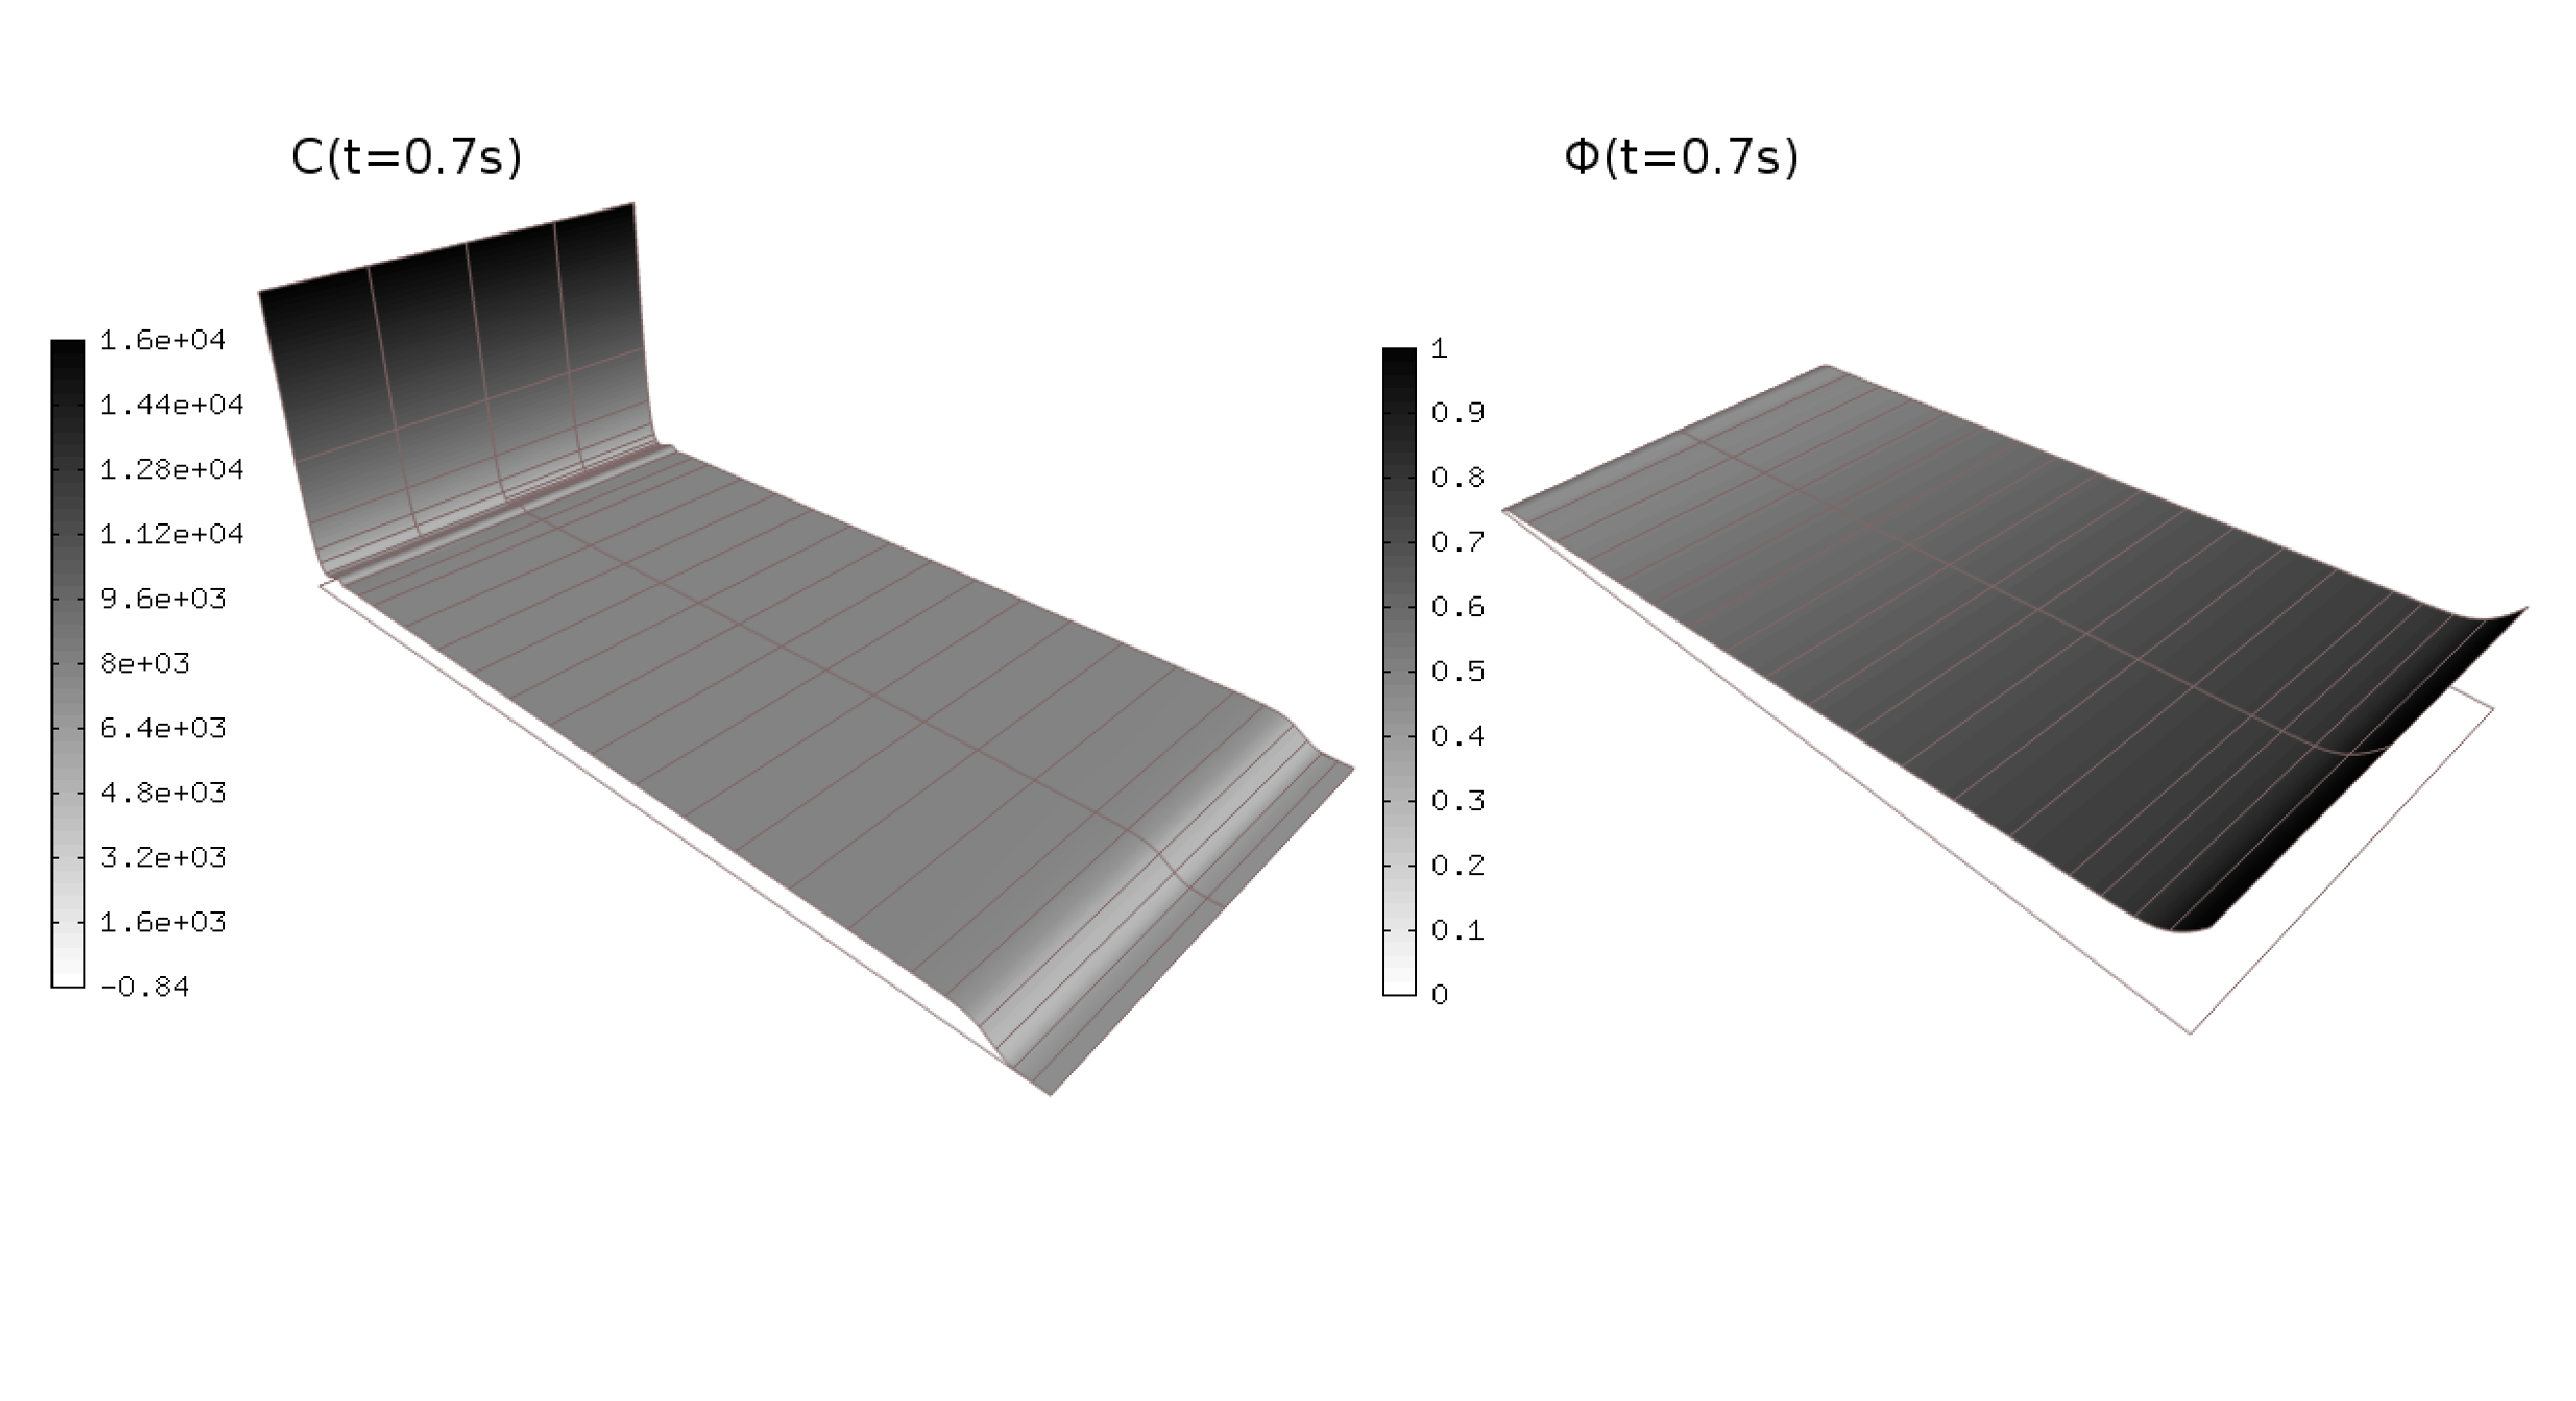
\includegraphics[width=\columnwidth]{cphi-1}
  \caption{\label{fig:cphi-1} Scaled concentration $c$
  and voltage $\varphi$ at $t=0.1\ s$.}
  \end{centering}
\end{figure}

%\newpage

\begin{figure}[!ht]
  \begin{centering}
  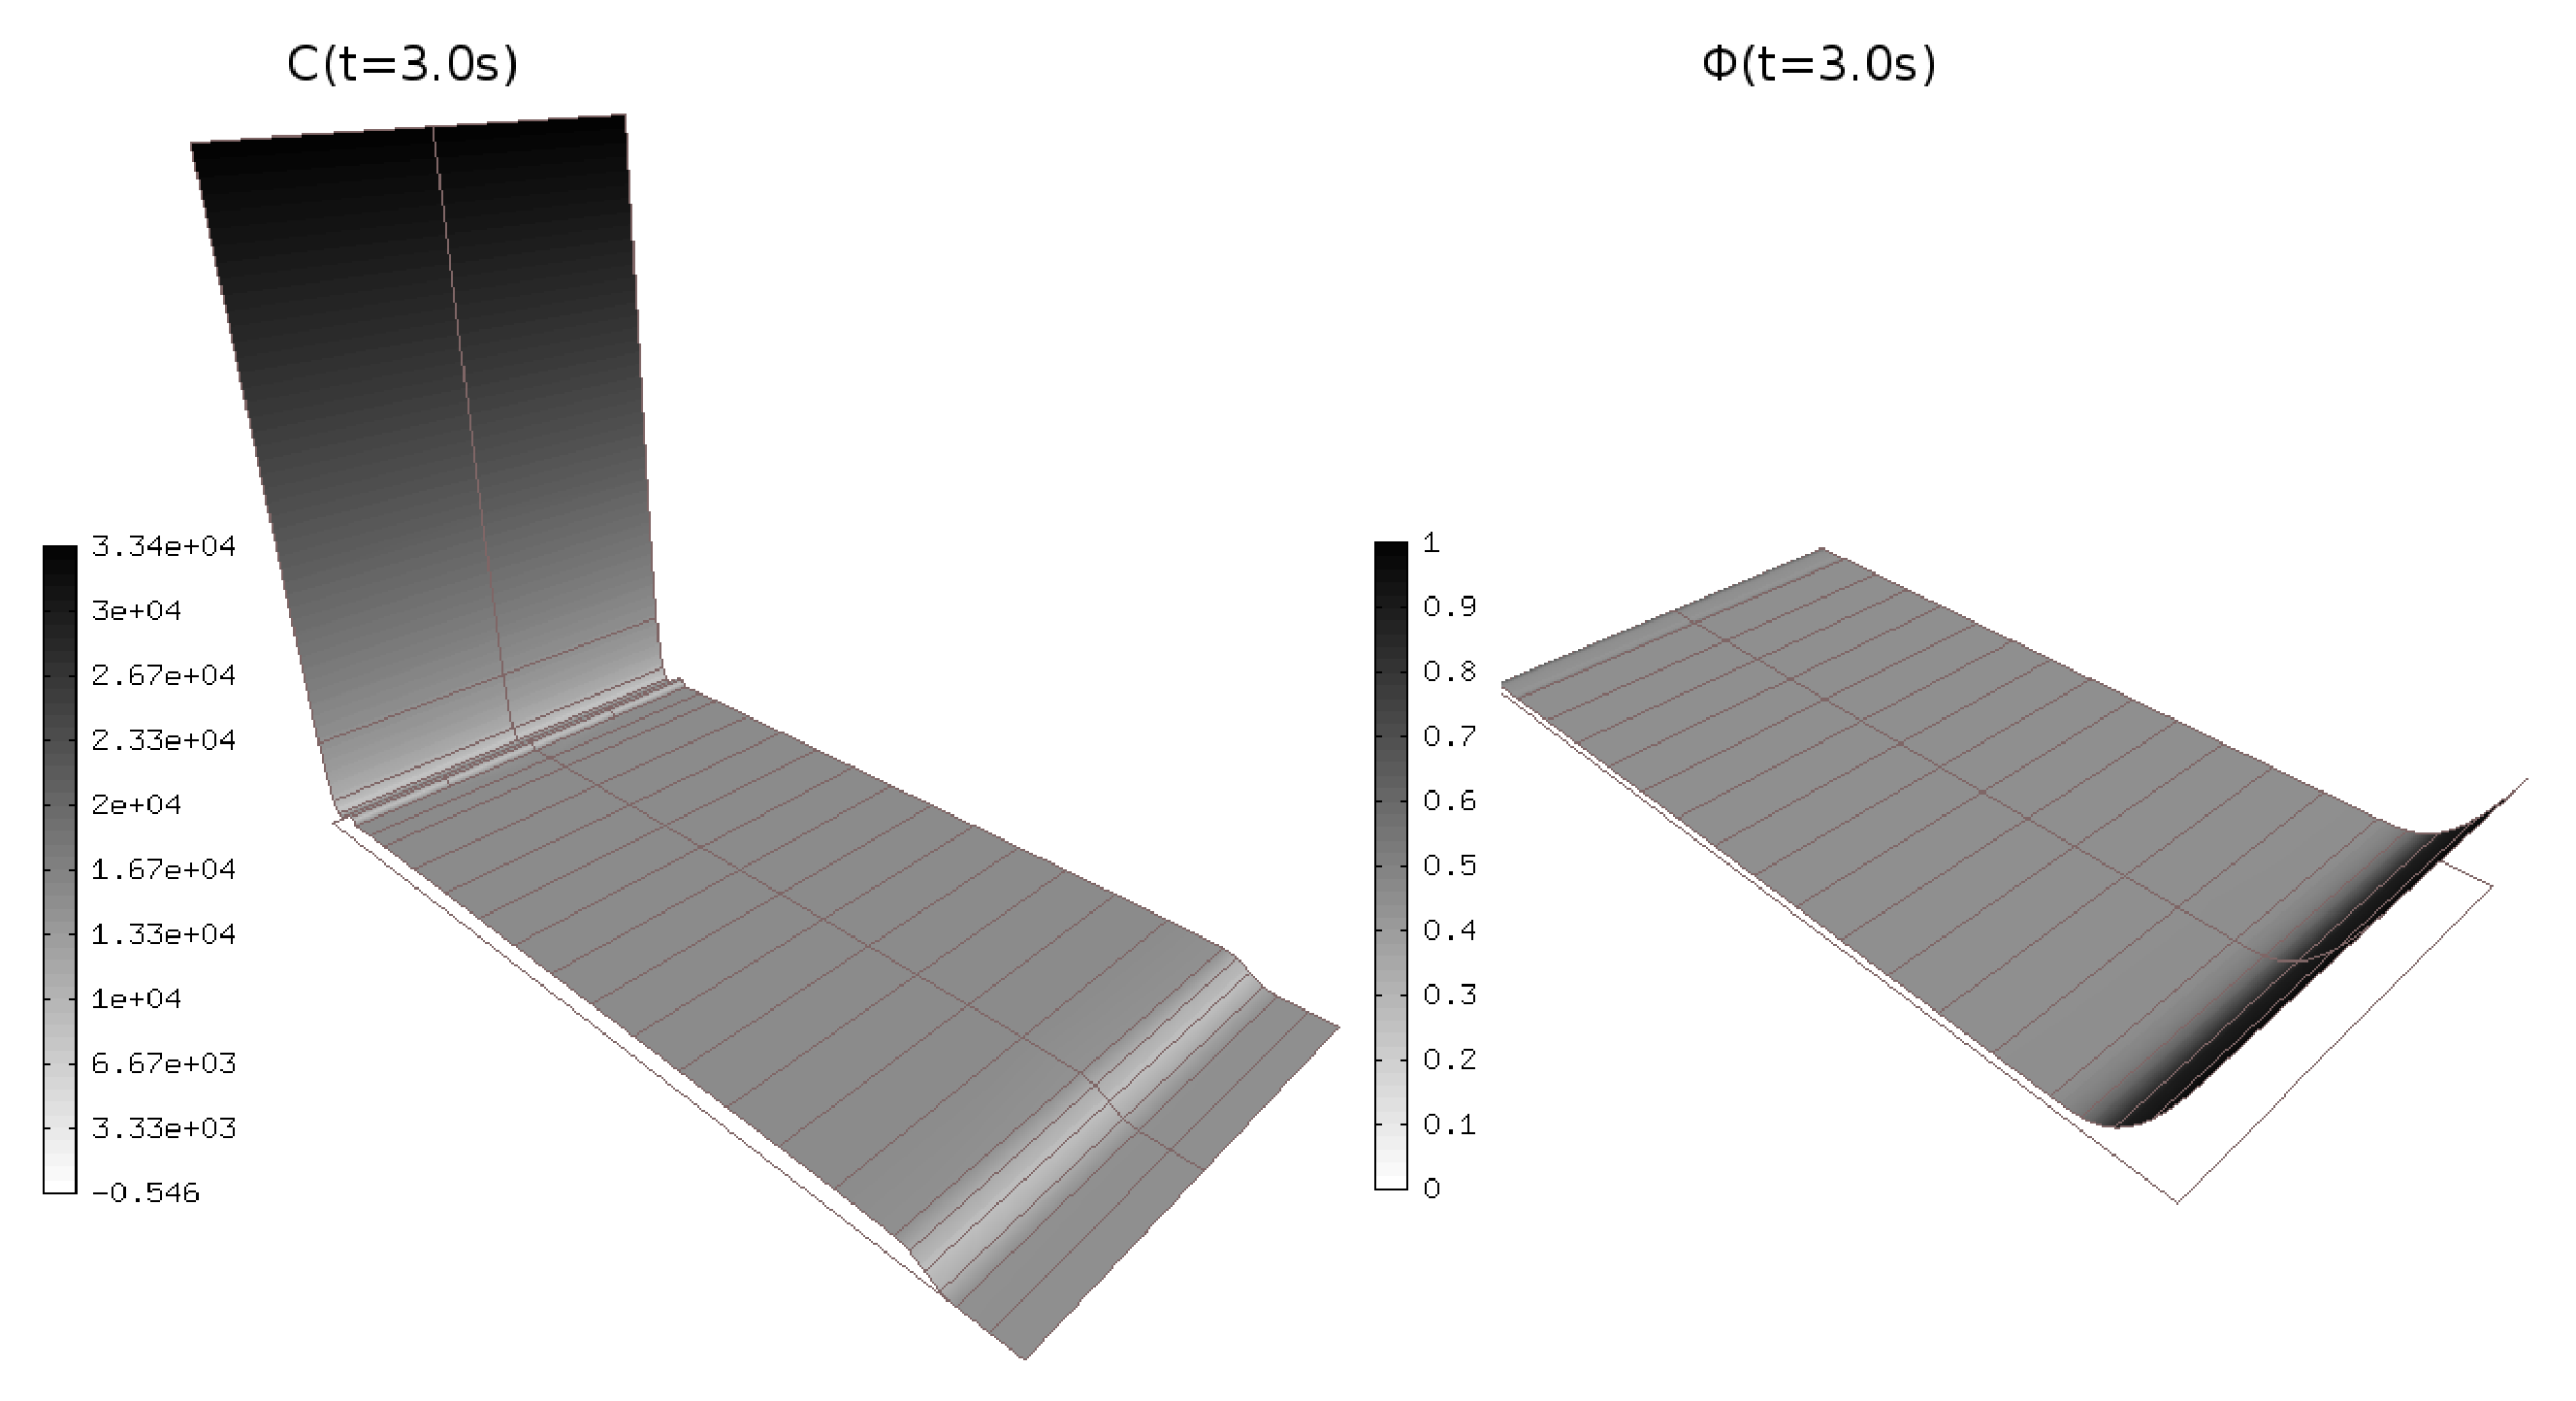
\includegraphics[width=\columnwidth]{cphi-2}
  \caption{\label{fig:cphi-2} Scaled concentration $c$
  and voltage $\varphi$ at $t=3.0\ s$.}
  \end{centering}
\end{figure}

The reader can see that at $t=0.1\ s$ some ionic migration has already 
taken place and large concentration gradients near the boundaries $\partial\Omega_1$ 
and $\partial\Omega_3$ have formed. The figures also show that the meshes 
at $t=0.1\ s$ and $t=3.0\ s$ are different. 

\subsection{Comparison of single mesh low-order FEM and $hp$-FEM}

First of all, the low-order FEM and $hp$-FEM were compared. A single mesh
H\_ANISO with polynomial degrees $p=1$ and $p=2$ were compared to
HP\_ANISO mode. The coarse initial mesh as shown in Fig.~\ref{fig:mesh}~(a)
was used in the solutions.
The results are shown in Figs.~\ref{fig:singlehhpdof} 
and~\ref{fig:singlehhpcpu}.
\begin{figure}[!ht]
  \begin{centering}
  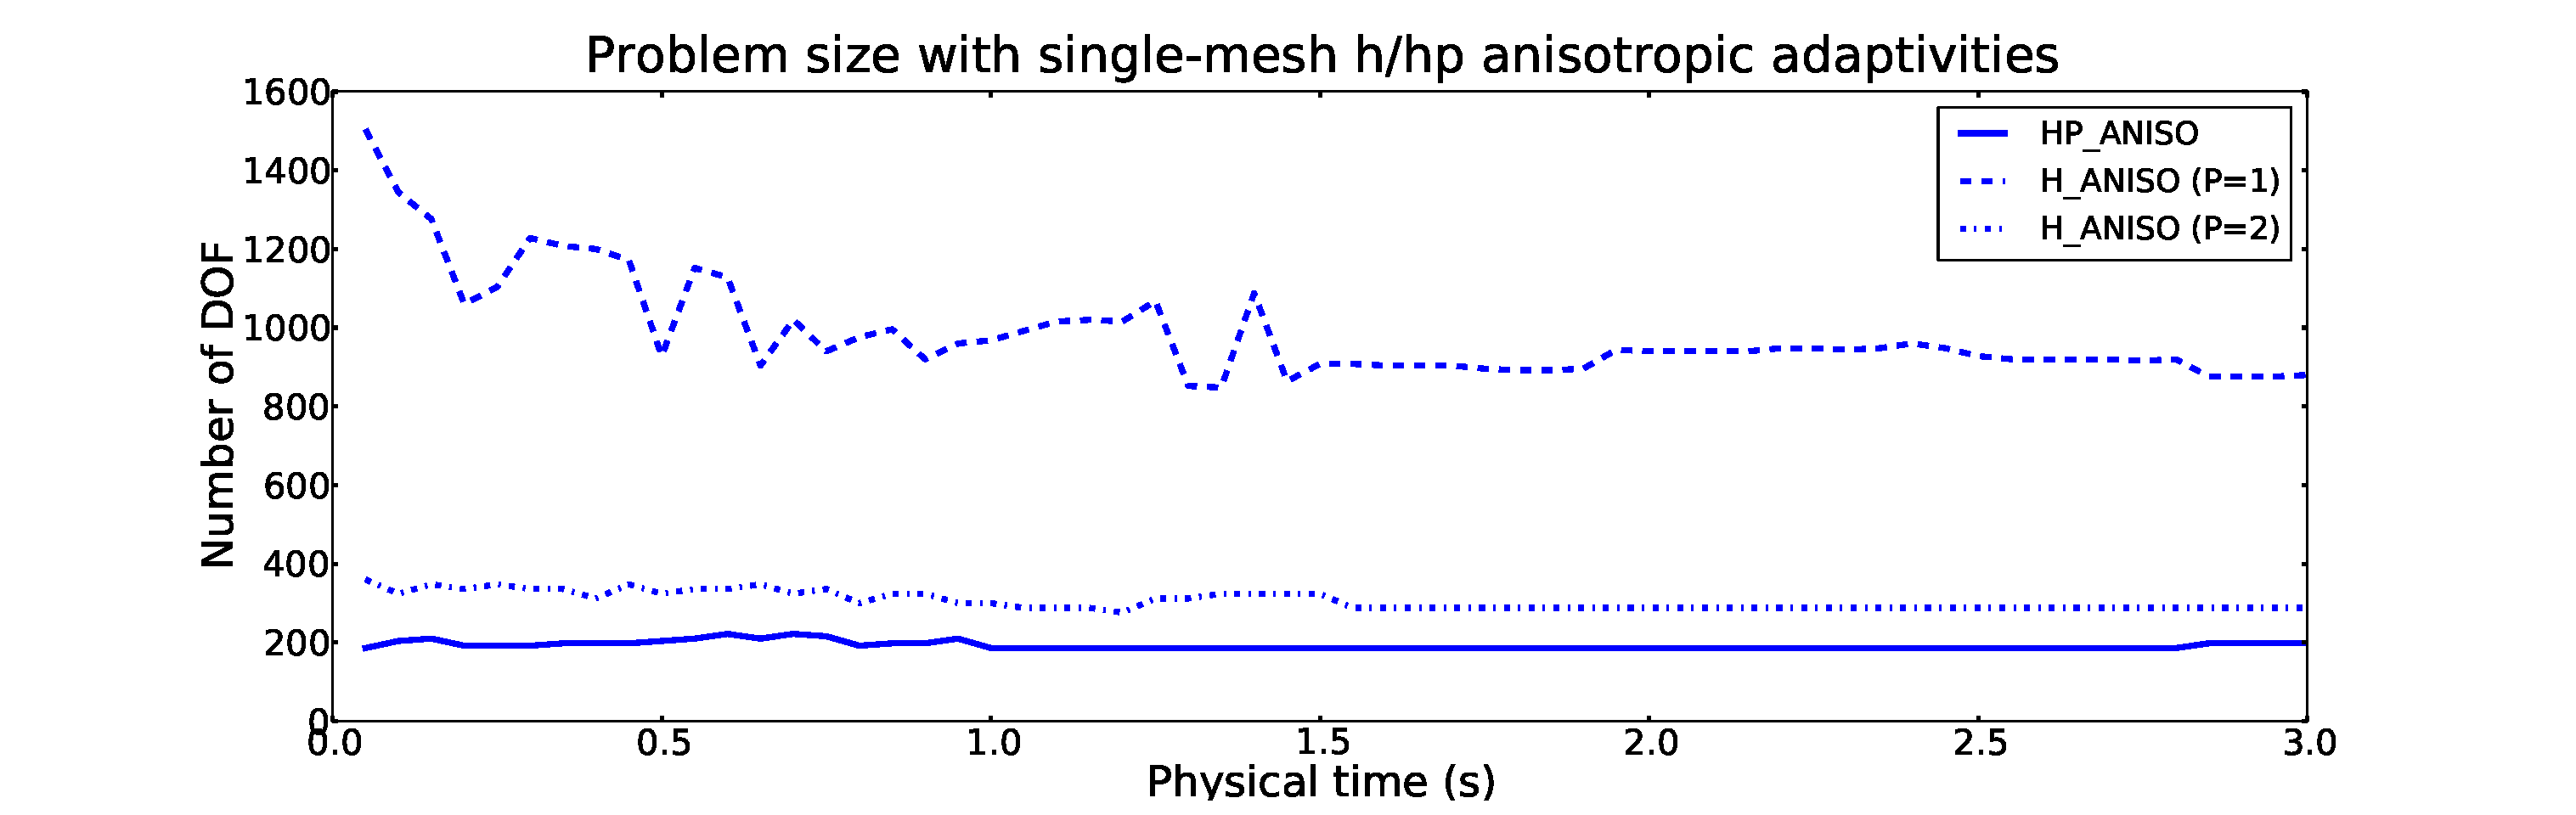
\includegraphics[width=\columnwidth]{singleh_hp_dof}
  \caption{\label{fig:singlehhpdof} Number of degrees of freedom (DOF) as a function 
  of physical time for single-mesh H\_ANISO (in case of
  $p=1$ and $p=2$) and single-mesh HP\_ANISO.}
  \end{centering}
\end{figure}


\begin{figure}[!ht]
  \begin{centering}
  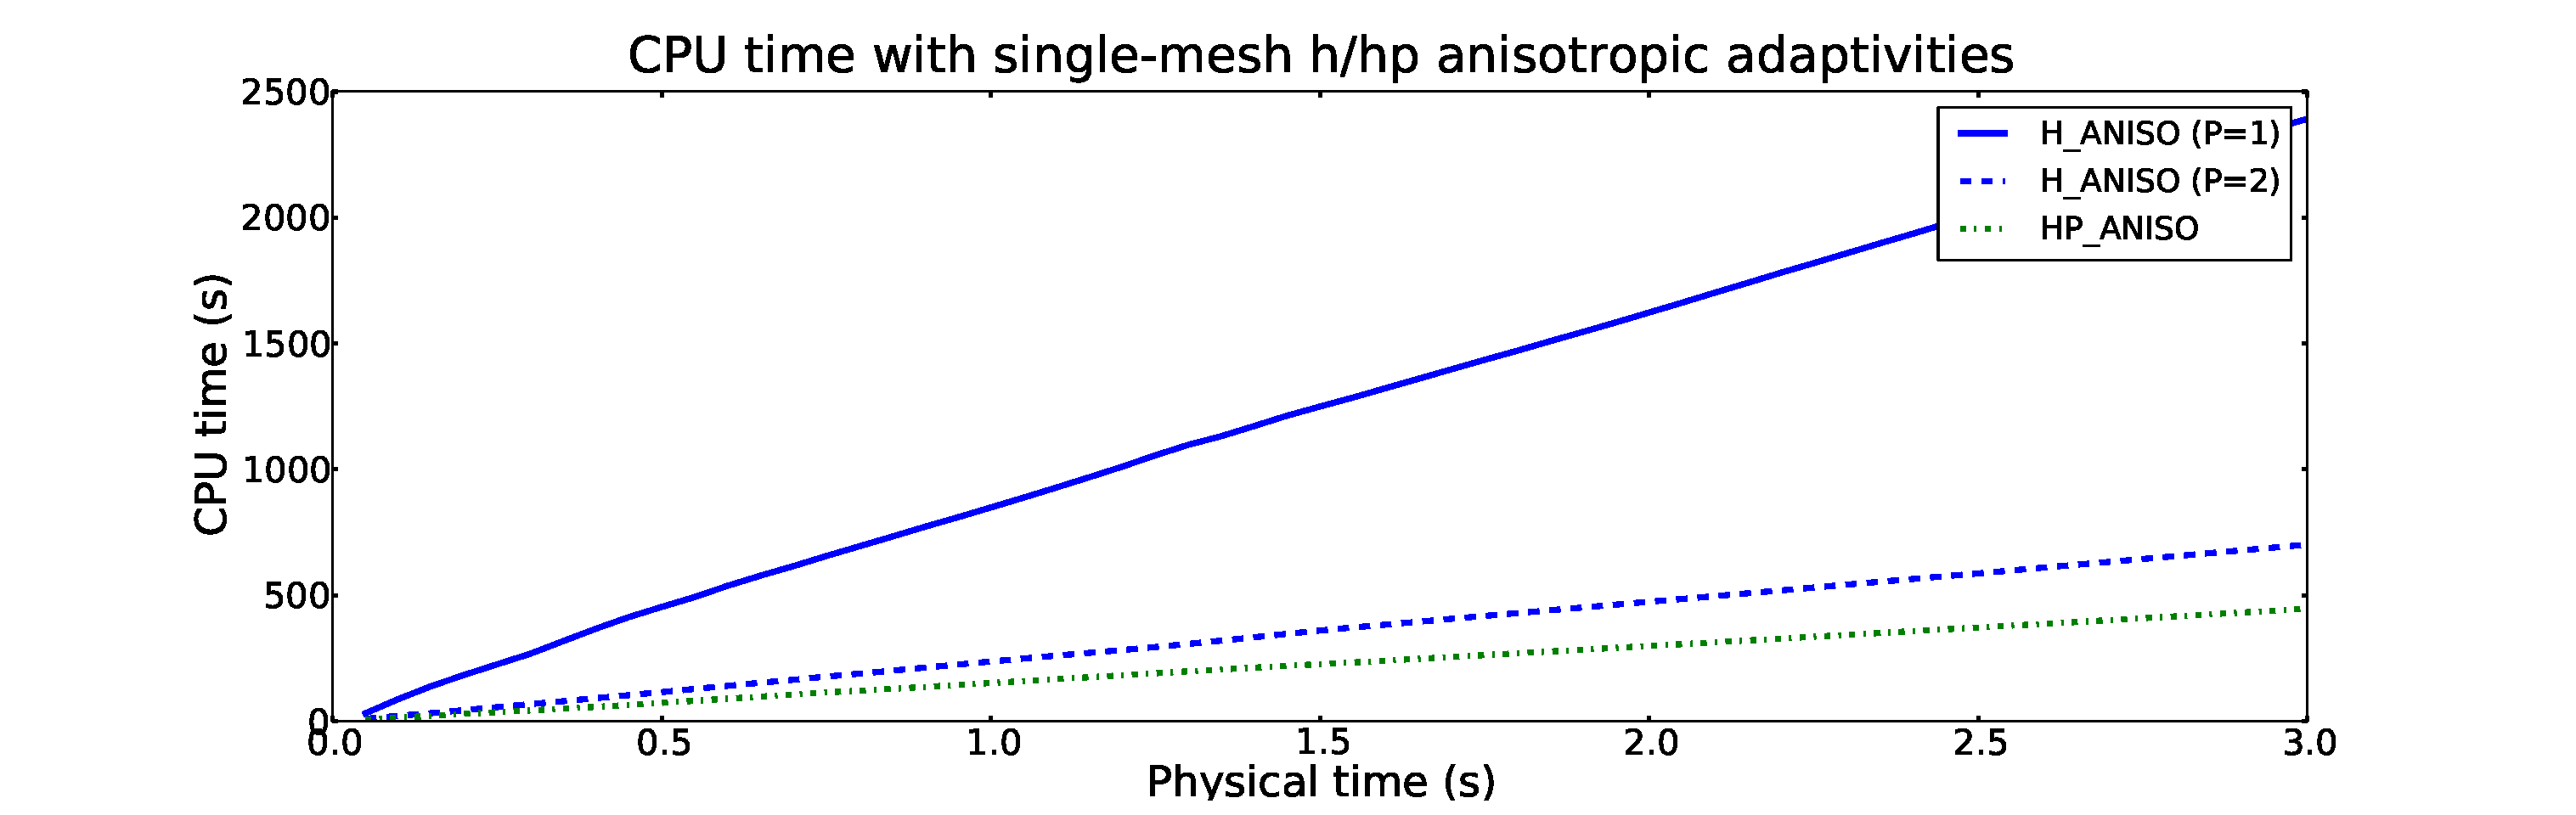
\includegraphics[width=\columnwidth]{singleh_hp_cpu}
  \caption{\label{fig:singlehhpcpu} Cumulative CPU time as a function 
  of physical time for single-mesh H\_ANISO (in case of $p=1$ and $p=2$)
  and single mesh HP\_ANISO.}
  \end{centering}
\end{figure}

\noindent
It can be seen that $hp$-FEM results in a shorter computing 
time and smaller number
of DOF than the low-order FEM. The same holds true
for H\_ISO and HP\_ISO modes. In fact, in case of H\_ISO the relative error did not
converge to the pre-set threshold value of $0.5\%$ within acceptable range 
of degrees of freedom of $nDOF_{threshold}=5000$.
Therefore, the $h$-FEM solutions will be omitted from the further comparisons.
Instead, only $hp$-FEM solutions on the coarse mesh and $p$-FEM solutions
on the fine mesh will be discussed.

\subsection{Comparison of single-mesh and multi-mesh $hp$-FEM}
% David: Error convergence plots here.
Running the simulation with different adaptivity modes 
and meshes showed that the multi-mesh $hp$-FEM configuration resulted in
the smallest problems and similar error 
convergence compared to any single-mesh configuration. However,
multi-mesh problems generally resulted in longer computing times. This is a known
shortcoming of Hermes at this point and it is due to the fact that
multi-mesh uses the union mesh (see Section~\ref{sec:hermes}) where 
the numerical integration of high order is done on very small elements.
The problem size and computing time are illustrated for HP\_ANISO adaptivity mode in Fig.~\ref{fig:singlemultidof} and Fig.~\ref{fig:singlemulticpu}.
The same holds true for HP\_ISO mode.  It must be also noted that the error
converged to or below $0.5\%$ for all $p$-FEM and anisotropic $hp$-FEM results.
 
\begin{figure}[!ht]
  \begin{centering}
  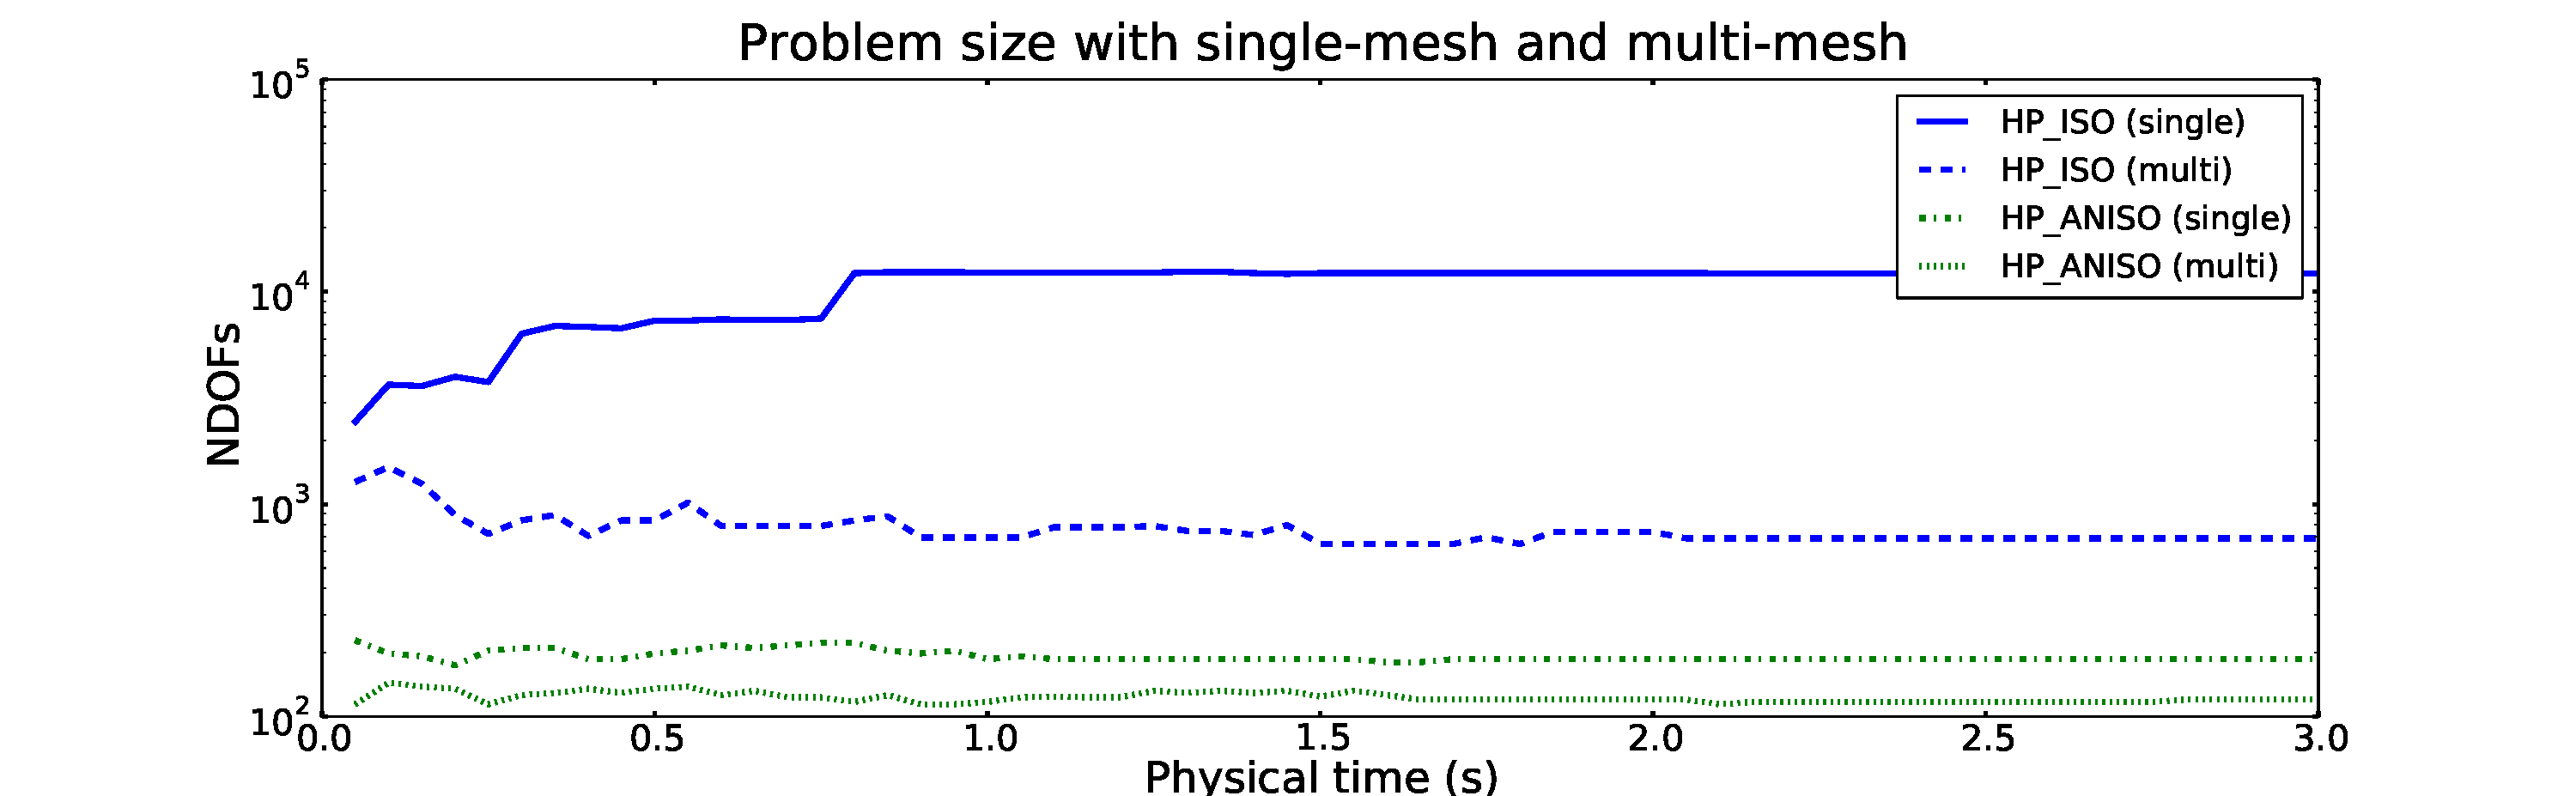
\includegraphics[width=\columnwidth]{singlemulti_dof}
  \caption{\label{fig:singlemultidof} Number of DOF as a function 
  of physical time for single-mesh and multi-mesh configurations with 
  HP\_ANISO adaptivity mode.}
%\vspace{-6mm}
  \end{centering}
\end{figure}


\begin{figure}[!ht]
  \begin{centering}
  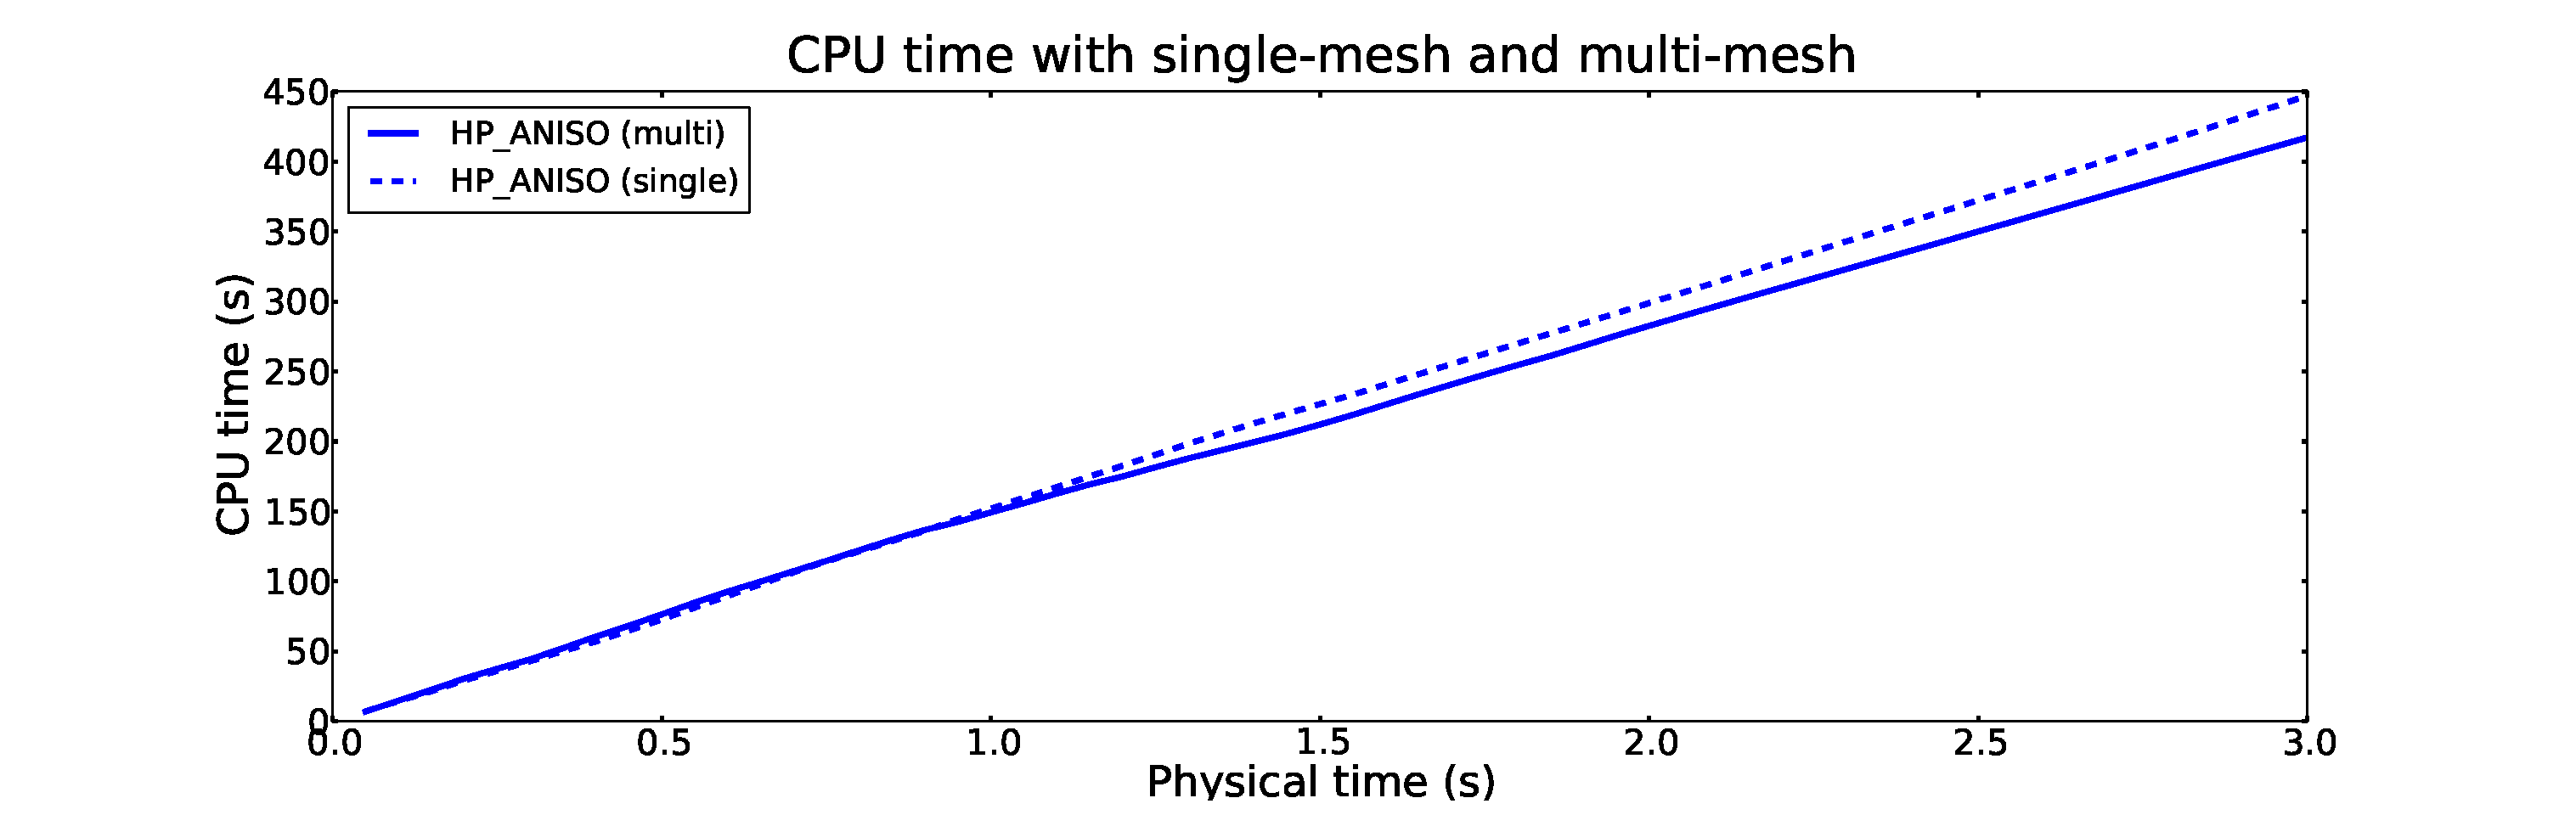
\includegraphics[width=\columnwidth]{singlemulti_cpu}
  \caption{\label{fig:singlemulticpu} Cumulative CPU time as a function 
  of physical time for single-mesh and multi-mesh configurations with 
  HP\_ANISO adaptivity mode.}
  \end{centering}
\end{figure}

\noindent 
Figs.~\ref{fig:poly} and~\ref{fig:poly2} show higher-order meshes in the adaptive multi-mesh $hp$-FEM
computation for $c$ and $\varphi$ at $t = 0.1$~s and $t=3.0$~s, respectively. Different 
colors mean different polynomial degrees. A diagonal pattern inside an element 
tells that the element has different polynomial degrees in the 
horizontal and vertical directions. 


\begin{figure}[!ht]
  \begin{centering}
  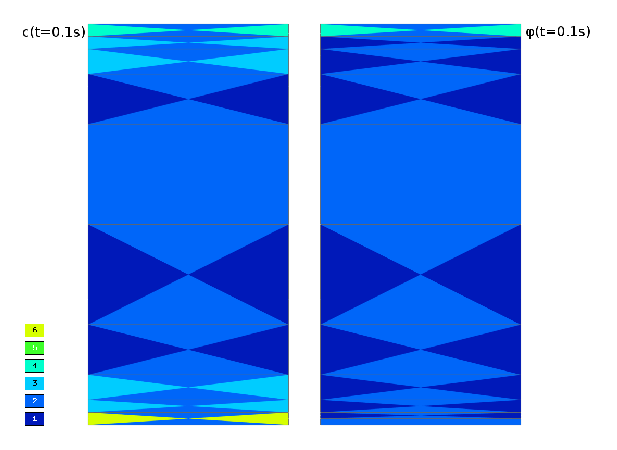
\includegraphics[width=.75\columnwidth]{poly}
  \caption{\label{fig:poly} Higher-order FEM mesh for 
  $c$ and $\varphi$ at $t=0.1\ s$. }
  \end{centering}
\end{figure}

\begin{figure}[!ht]
  \begin{centering}
  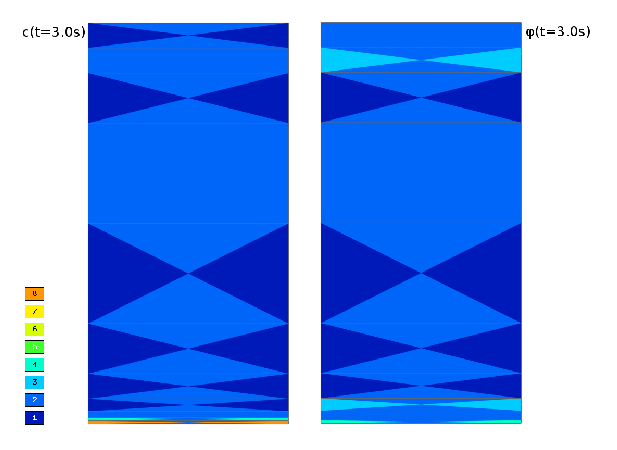
\includegraphics[width=.75\columnwidth]{poly2}
  \caption{\label{fig:poly2} Higher-order FEM mesh for 
  $c$ and $\varphi$ at $t=3.0\ s$. }
  \end{centering}
\end{figure}
\noindent
The result are in good agreement with Fig.~\ref{fig:cphi-2} --- in the vicinity
of the boundaries $\partial \Omega_1$ and $\partial\Omega_3$, the concentration gradient
is much greater than the voltage gradient. Therefore at $t=0.1$~s, 
the multi-mesh $hp$-FEM adaptivity 
algorithm has increased the maximum polynomial degree for the $c$-space to~6 while 
the maximum polynomial degree for the $\varphi$-space is~4. The meshes are not
that different in the beginning of the calculation. However, one can also see that the mesh 
refinement for $c$ at $t=3.0$~s is notably different compared to $\varphi$. For instance,
the highest polynomial degree for $c$-space is~8 whereas for $\varphi$-space is~4.
Since these results are representative for all adaptivity modes, only multi-mesh 
configurations are considered in the following. 

\subsection{Comparison of isotropic and anisotropic refinements}

Next we would like to illustrate the role of anisotropic mesh refinements.
Figs.~\ref{fig:isoanisodof} and \ref{fig:isoanisocpu} show typical results 
for the HP\_ISO, HP\_ANISO\_H,  HP\_ANISO adaptivity modes in terms 
of DOF and cumulative CPU time. Fig.~\ref{fig:isoanisoerror} shows corresponding
error convergence. It can be seen that HP\_ISO is notoriously inefficient as the
error does not converge within the limited number of degrees of freedom 
of $nDOF_{threshold}=5000$ and computing time is very large. Due to that fact,
the calculation of HP\_ISO was canceled before $t=3.0$~s.

\begin{figure}[!ht]
  \begin{centering}
  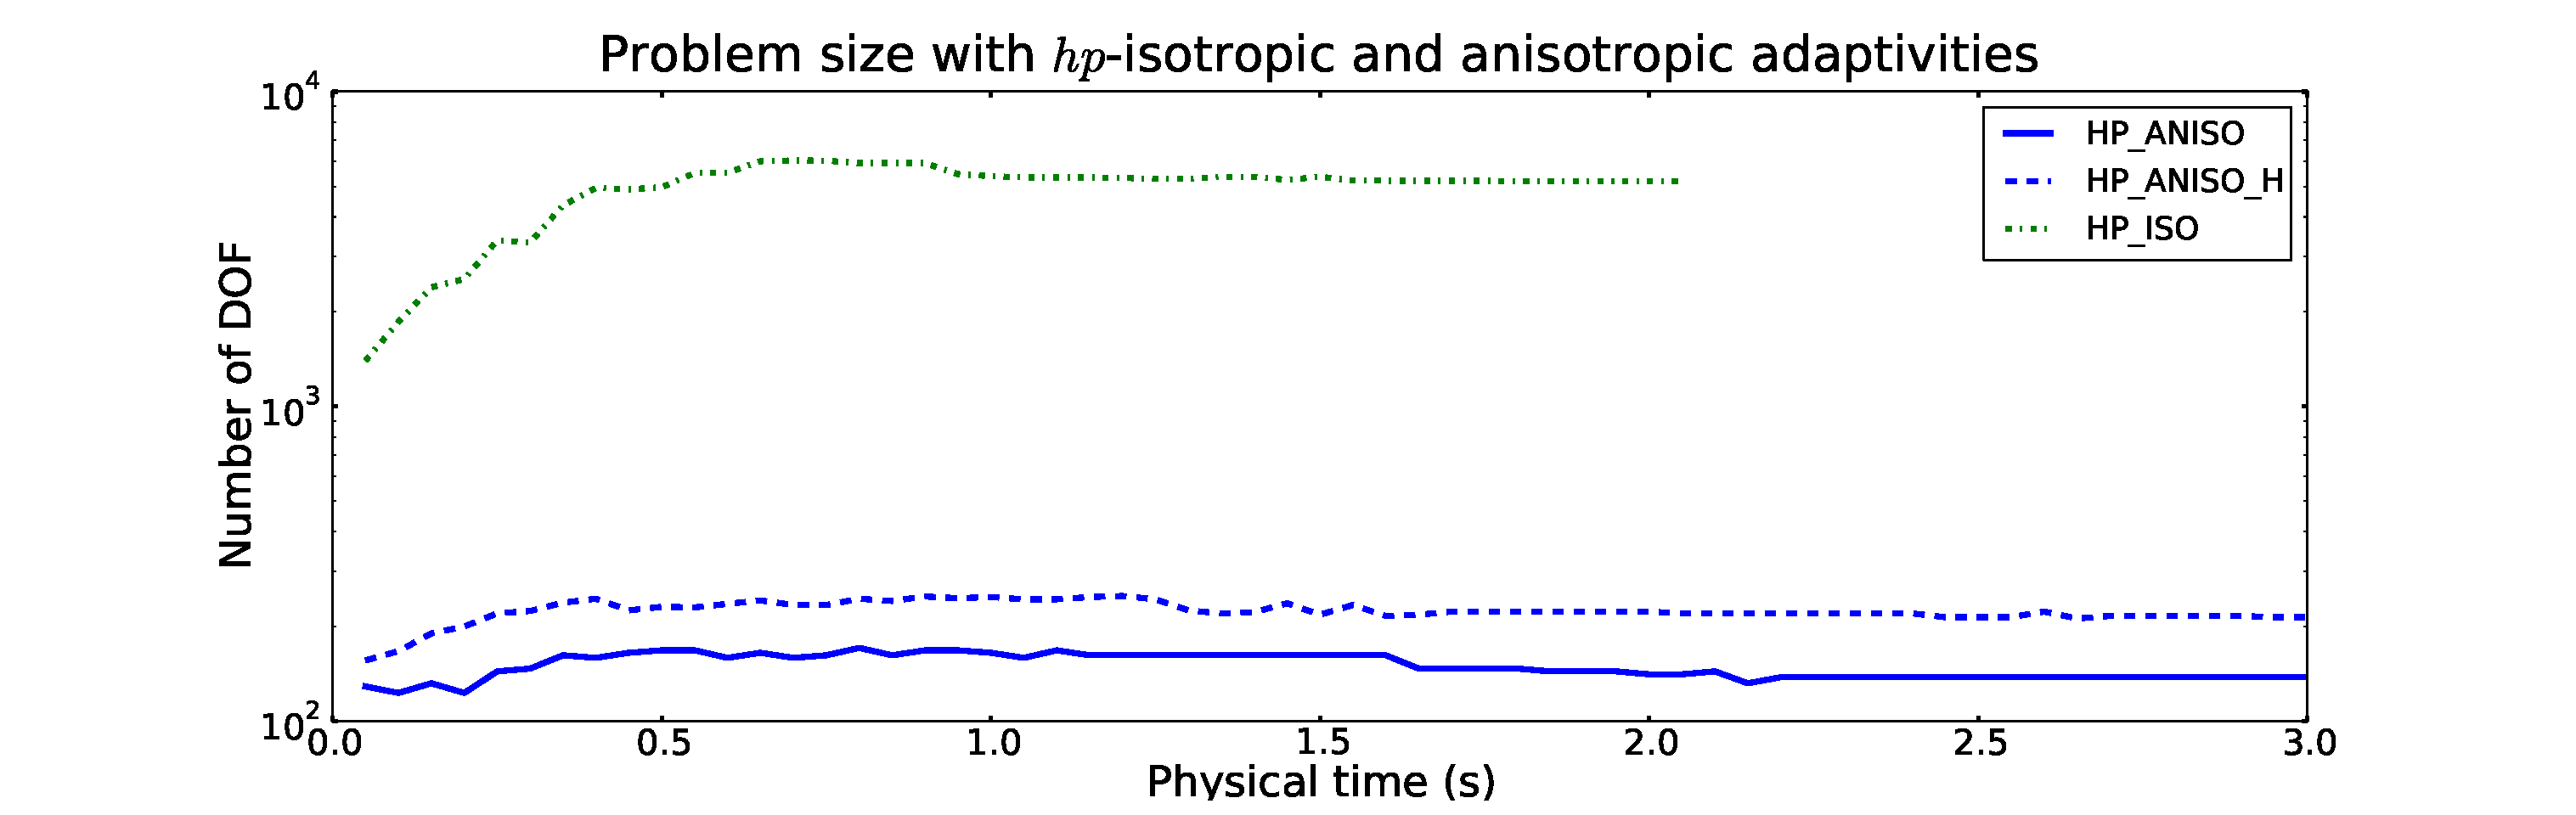
\includegraphics[width=\columnwidth]{isoaniso_dof}
  \caption{\label{fig:isoanisodof} Number of DOF as a function of physical time for 
  multi-mesh configurations with HP\_ANISO,
  HP\_ANISO\_H, and HP\_ISO adaptivity modes (log~$y$ scale).}
  \end{centering}
\end{figure}

\begin{figure}[!ht]
  \begin{centering}
  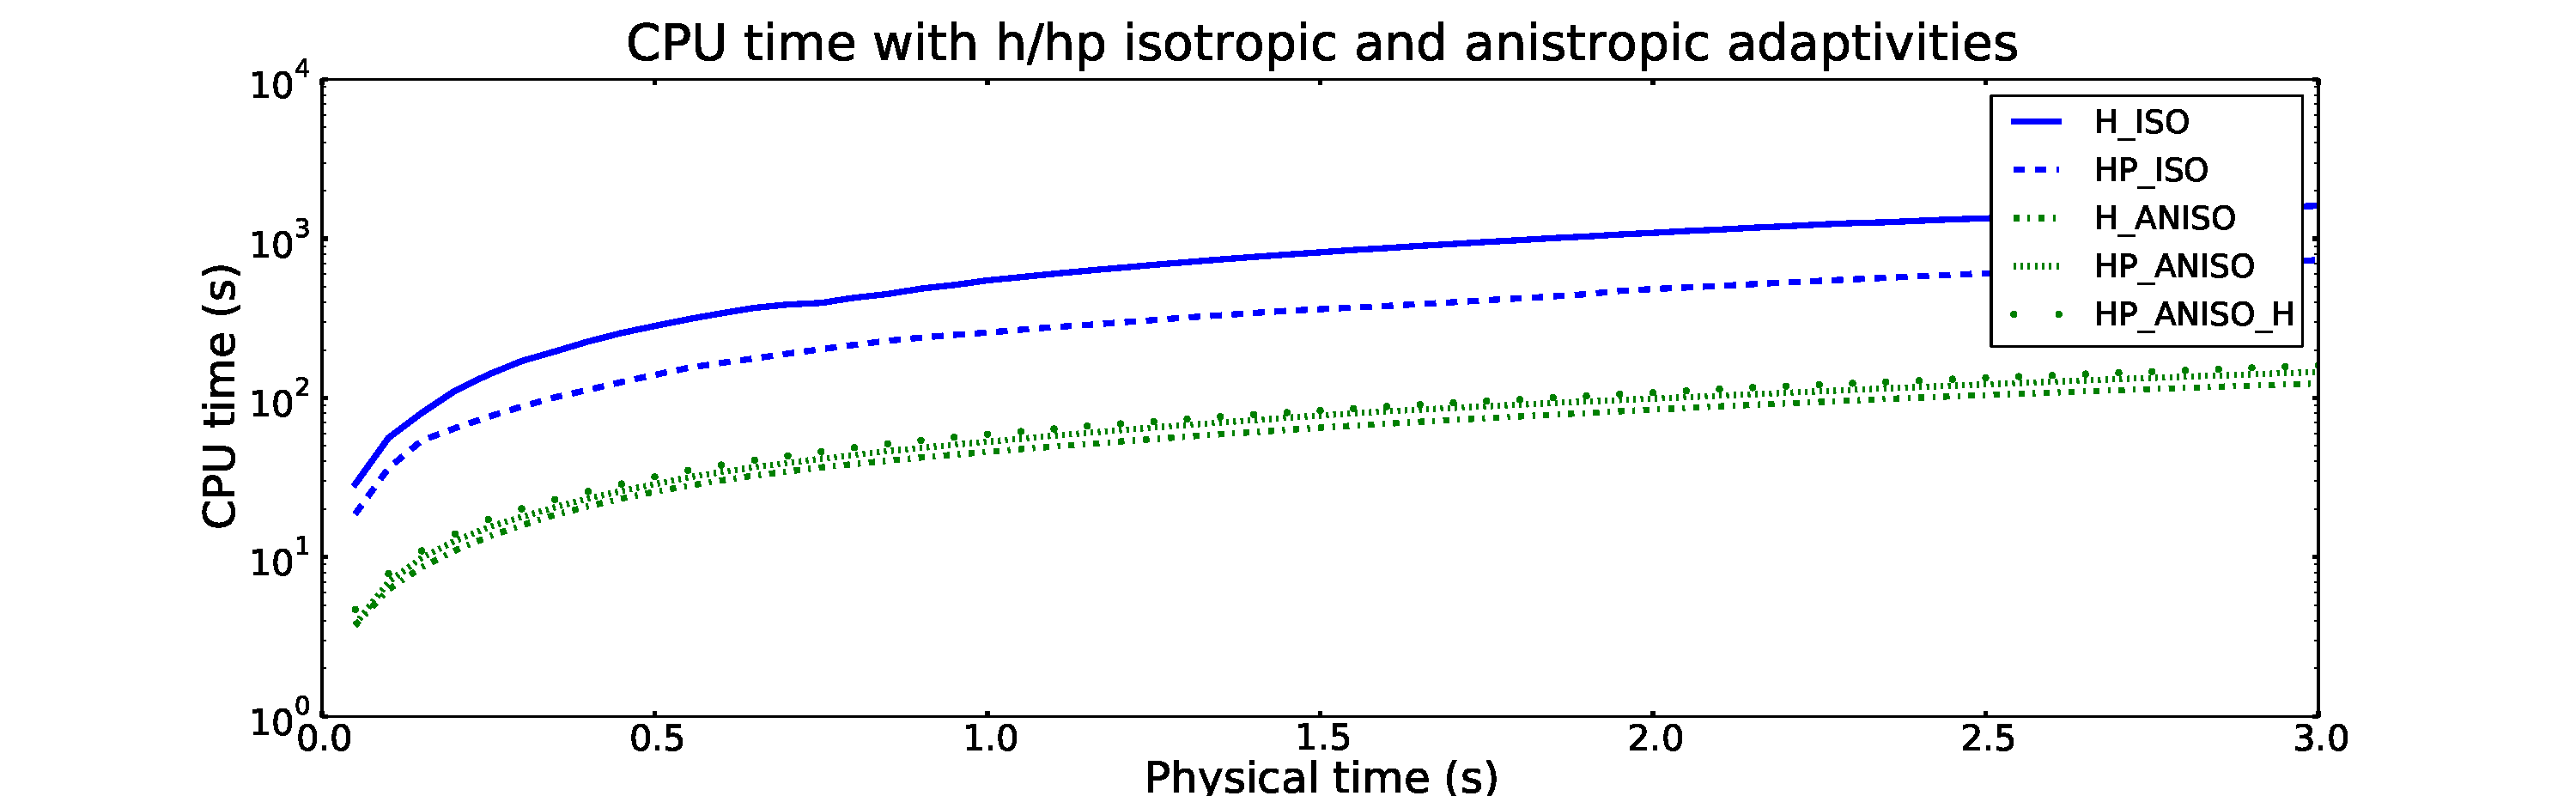
\includegraphics[width=\columnwidth]{isoaniso_cpu}
  \caption{\label{fig:isoanisocpu} Cumulative CPU time as a function of physical time 
  for multi-mesh configurations with HP\_ANISO,
  HP\_ANISO\_H, and HP\_ISO adaptivity modes (log~$y$ scale).}
  \end{centering}
\end{figure}

\begin{figure}[!ht]
  \begin{centering}
  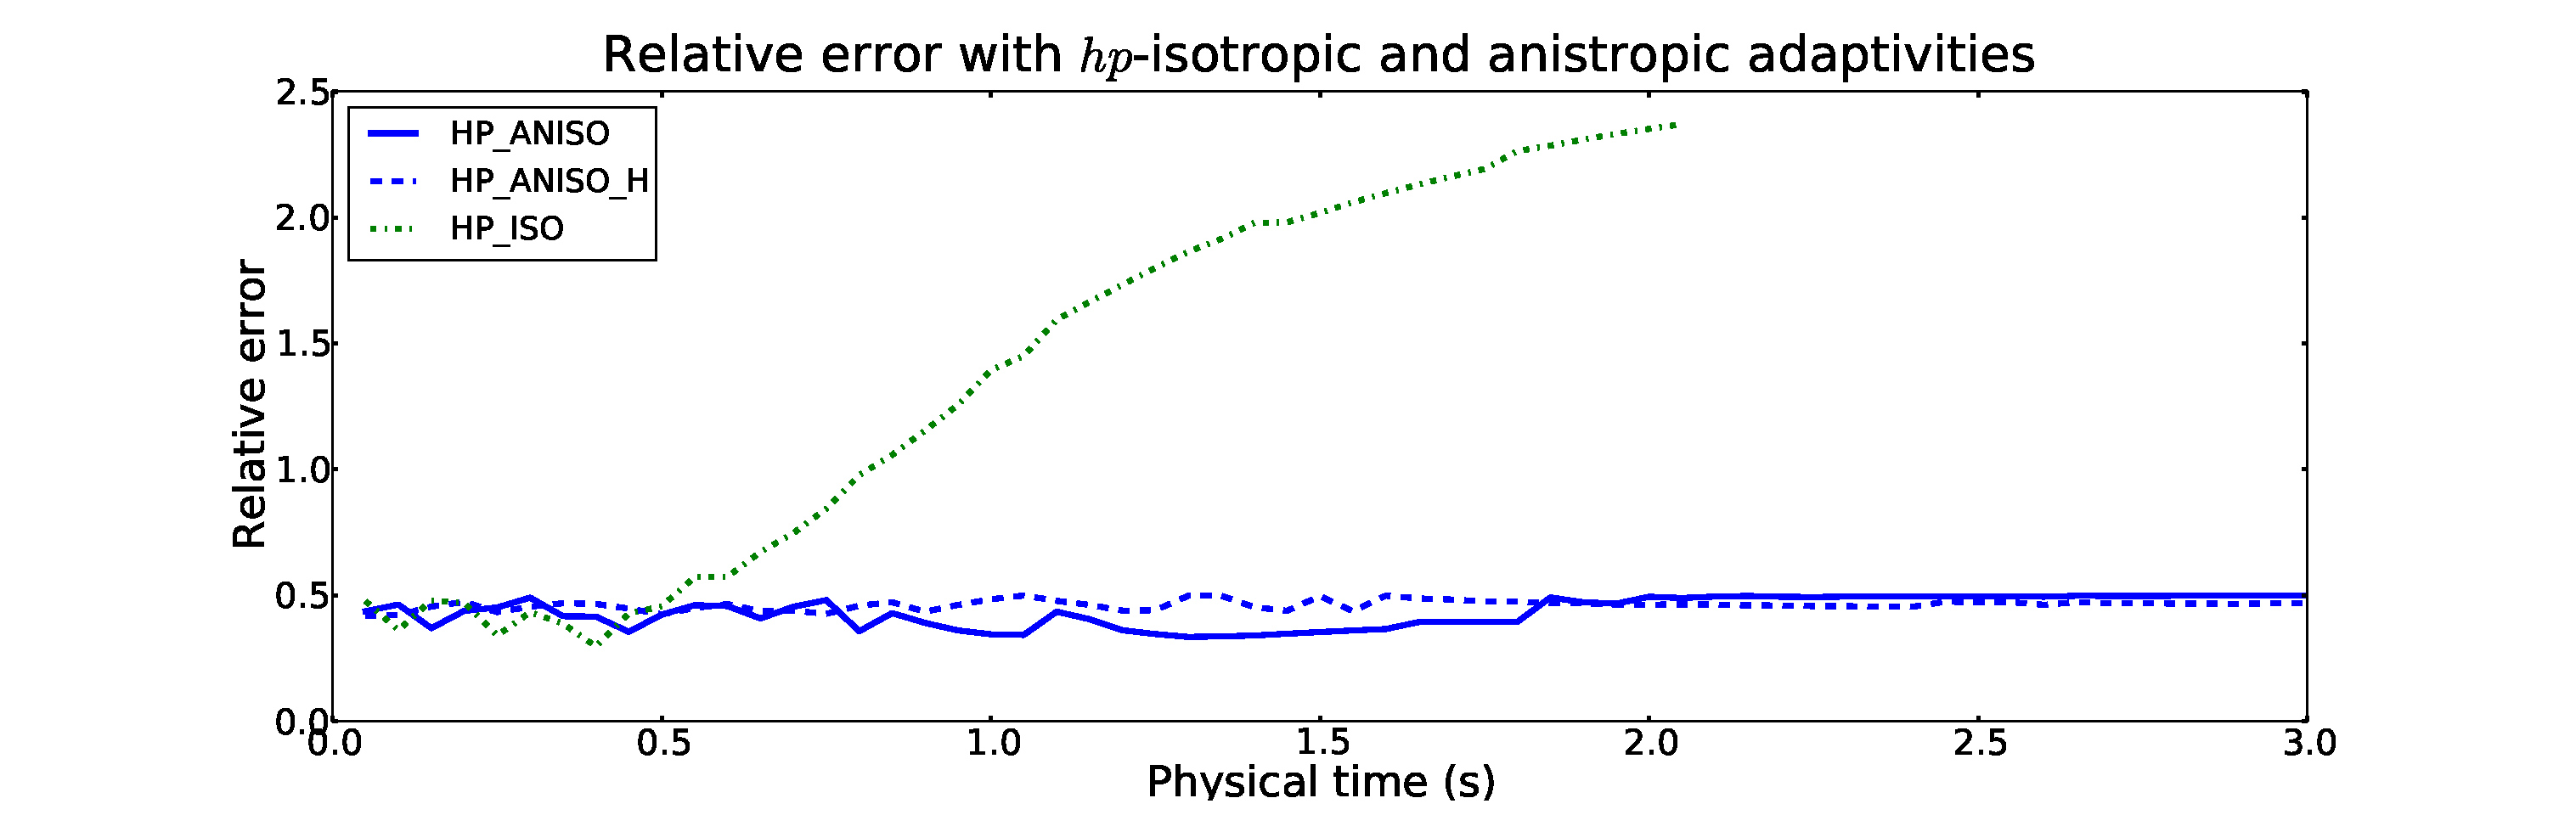
\includegraphics[width=\columnwidth]{isoaniso_error}
  \caption{\label{fig:isoanisoerror} Relative solution error as a function of physical time 
  for multi-mesh configurations with HP\_ANISO,
  HP\_ANISO\_H, and HP\_ISO adaptivity modes.}
  \end{centering}
\end{figure}

\noindent
Figs.~\ref{fig:isoanisopdof} and \ref{fig:isoanisopcpu} present a similar 
comparsion for the P\_ISO, P\_ANISO, and HP\_ANISO\_P modes. Recall that these 
computations use a different initial mesh that was a-priori refined in space.

%\newpage

\begin{figure}[!ht]
  \begin{centering}
  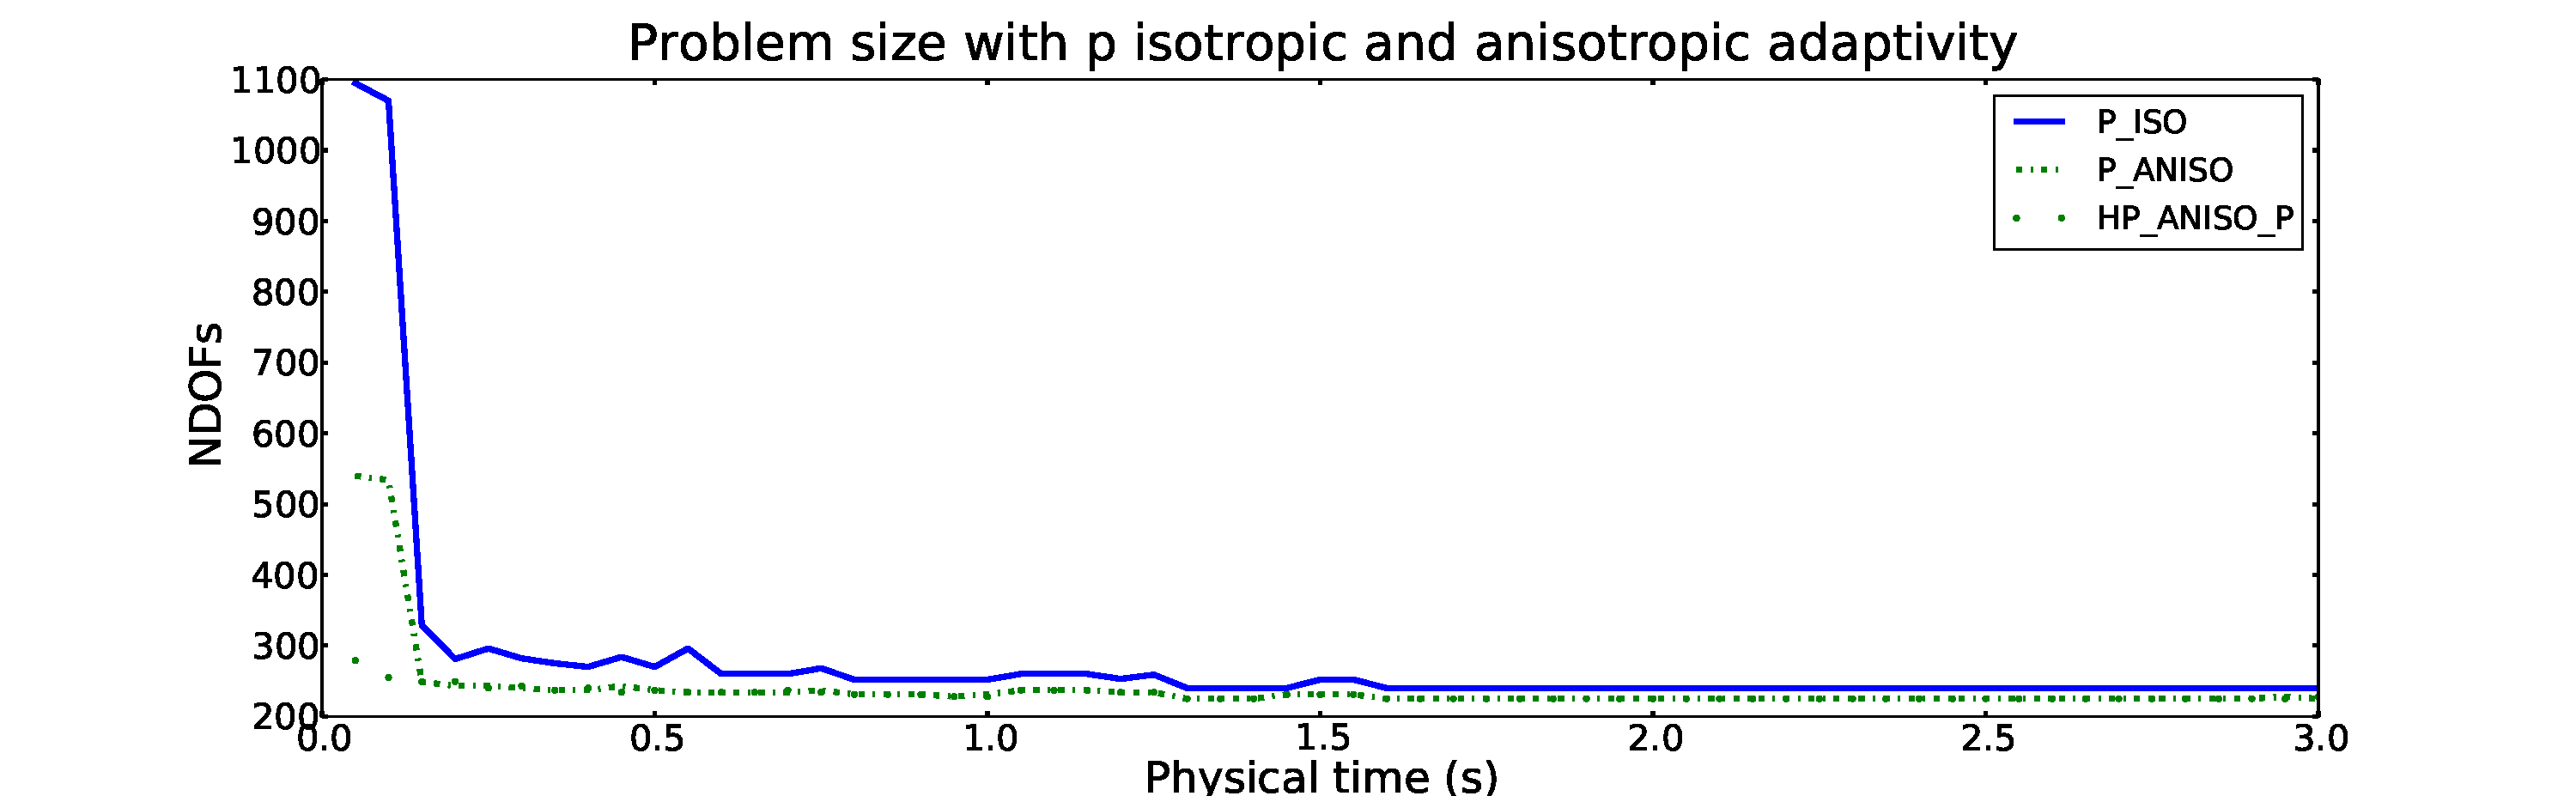
\includegraphics[width=\columnwidth]{isoanisop_dof}
  \caption{\label{fig:isoanisopdof} Number of DOF as a function of physical time
  for multi-mesh configurations with P\_ISO, P\_ANISO, and
  HP\_ANISO\_P adaptivity modes.}
  \end{centering}
\end{figure}

\begin{figure}[!ht]
  \begin{centering}
  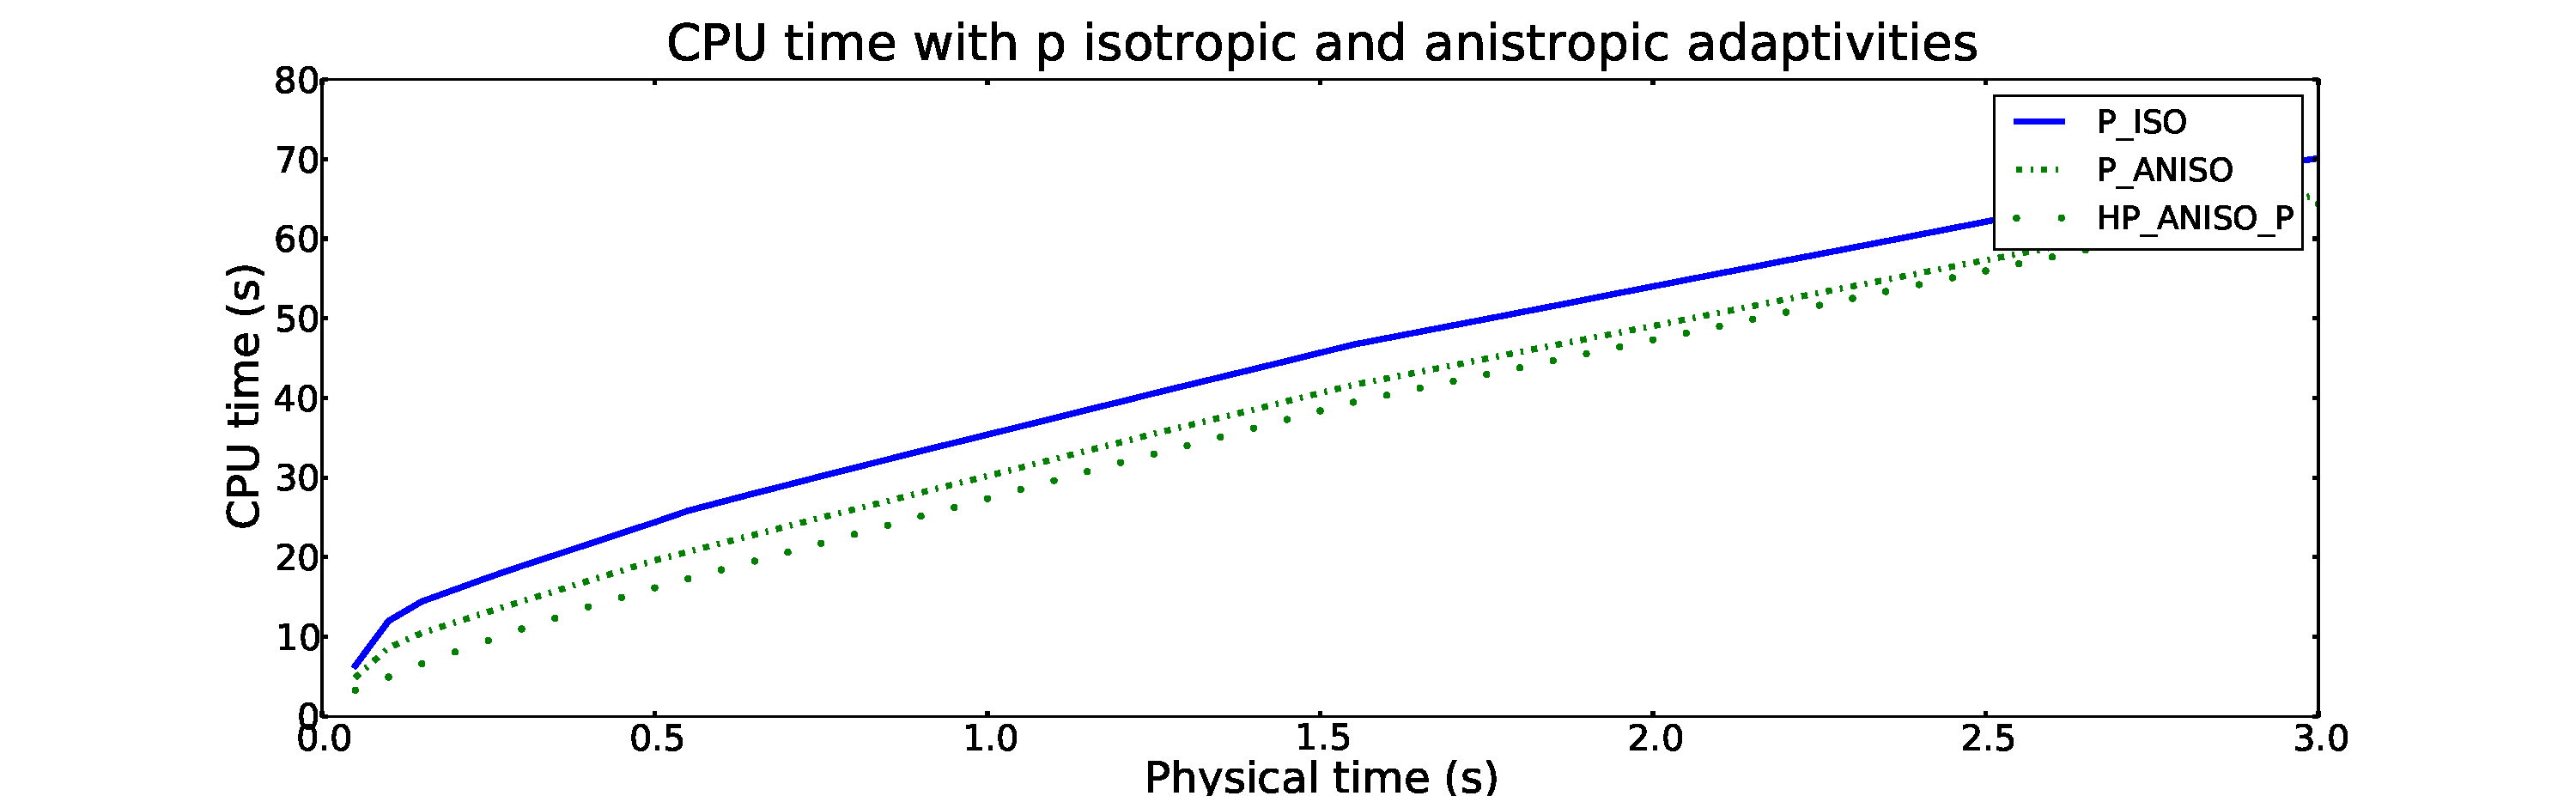
\includegraphics[width=\columnwidth]{isoanisop_cpu}
  \caption{\label{fig:isoanisopcpu} Cumulative CPU times as a function of physical time
  for multi-mesh configurations with P\_ISO, P\_ANISO, and
  HP\_ANISO\_P adaptivity modes.}
  \end{centering}
\end{figure}

As a conclusion, the reader can see that the anisotropic adaptivity modes always perform better than 
the isotropic ones. In particular, HP\_ANISO results into the smallest problem size. 
In the \emph{p}-adaptivity group, HP\_ANISO\_P and P\_ANISO lead to a small problem size
consistently in each time step, whereas P\_ISO yields large problems
during the first time steps. 

HP\_ANISO also results in the fastest
computing time among $hp$-adaptivity group whereas HP\_ANISO\_P
results in the fastest overall computing time. This is due to the fact
that HP\_ANISO\_P calculation is performed on the refined mesh. 
Regardless, the HP\_ANISO adaptivity mode is the most suitable
for the PNP problem due to the small size and relative fastness compared
to the other adaptivity modes. A way to optimize the computing time
of HP\_ANISO will be considered next.

\subsection{Time step control of HP\_ANISO adaptivity}

\begin{figure}[!ht]
  \begin{centering}
  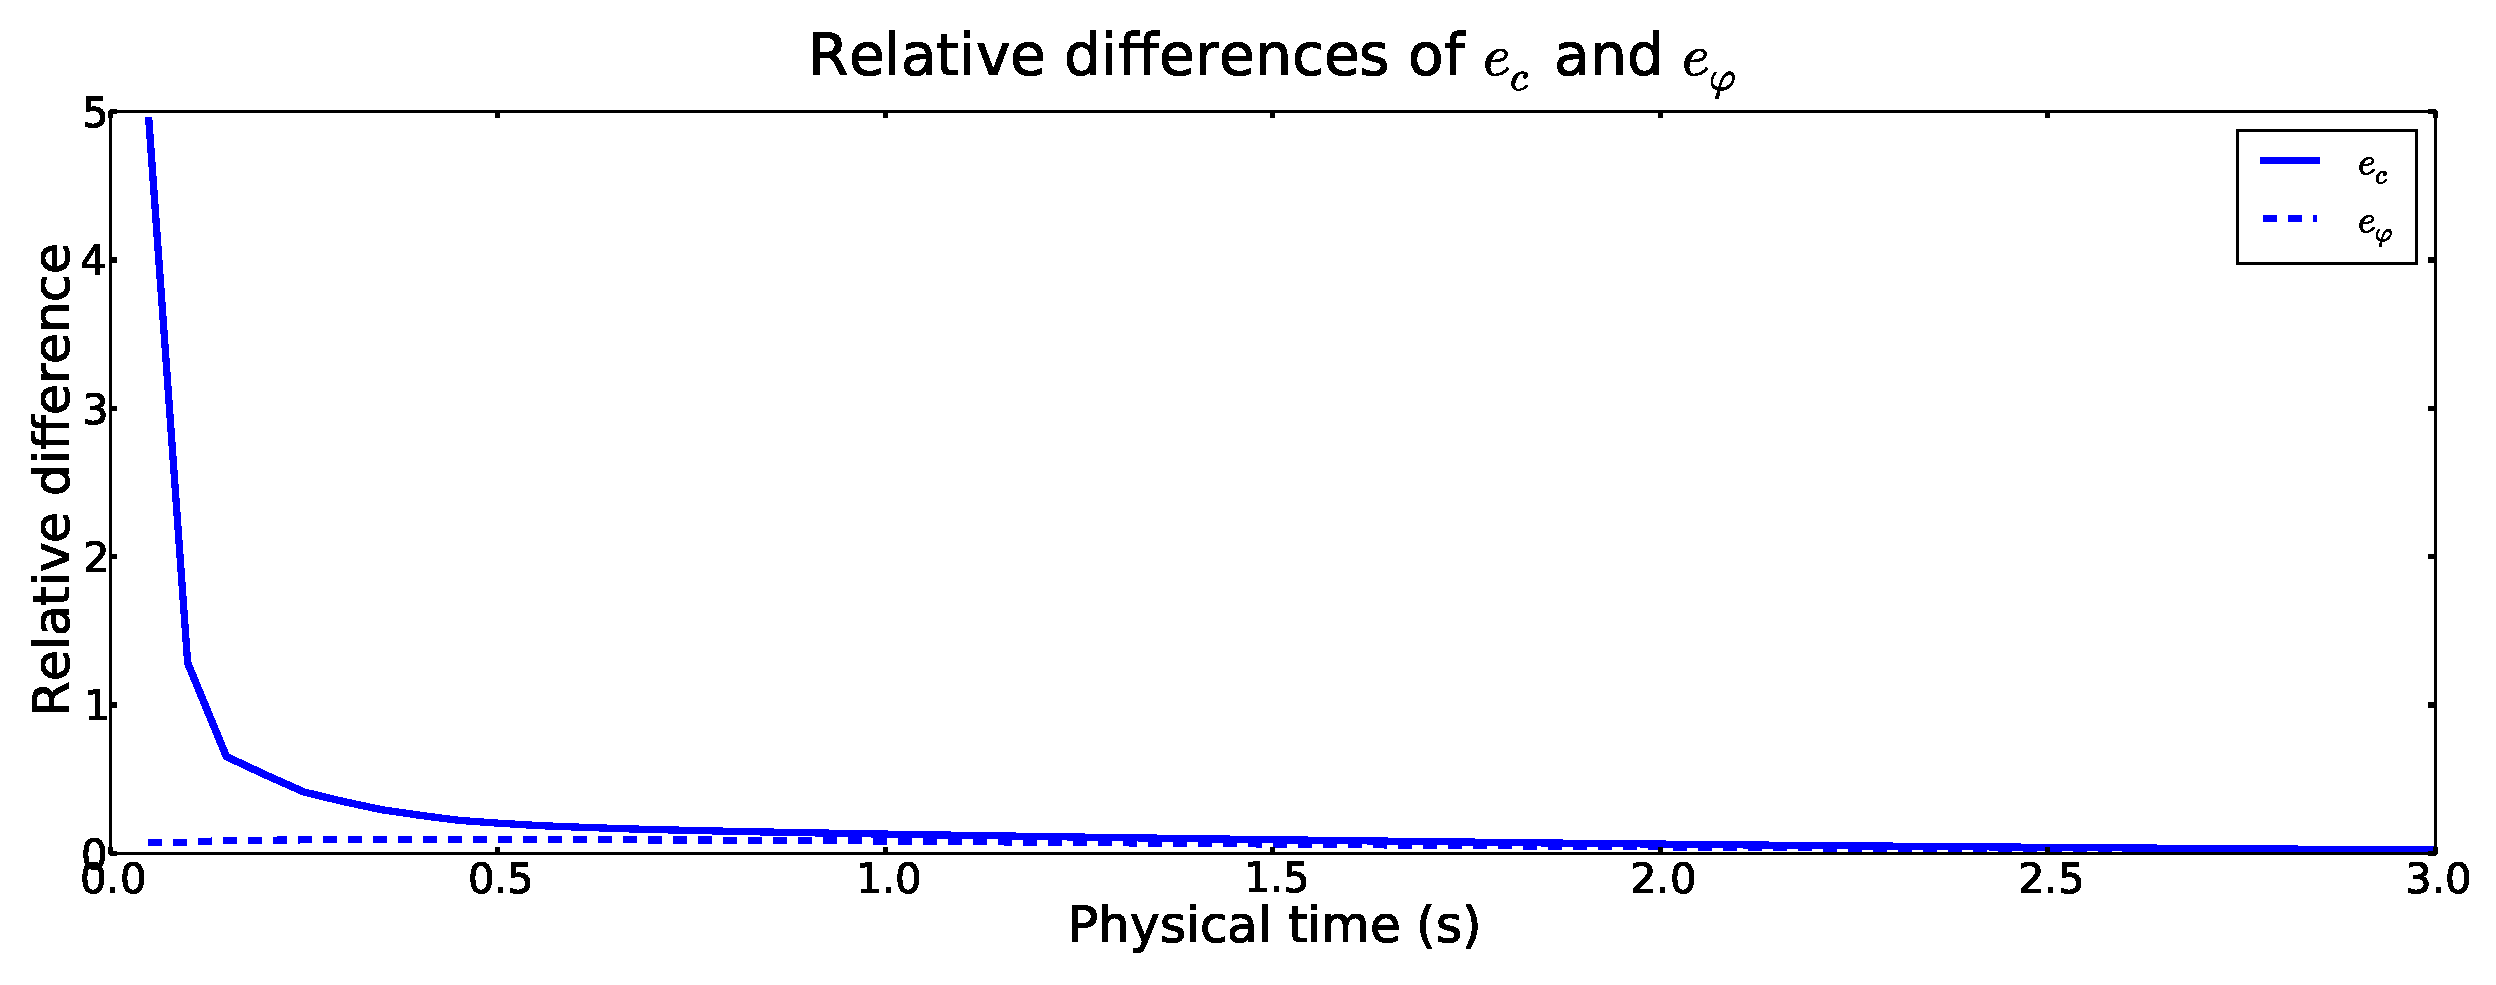
\includegraphics[width=\columnwidth]{cphi_relerr}
  \caption{\label{fig:cphirelerr} Relative difference $e_{c}^n$ and $e_{\varphi}^n$.}
  \end{centering}
\end{figure}
\begin{figure}[!ht]
  \begin{centering}
  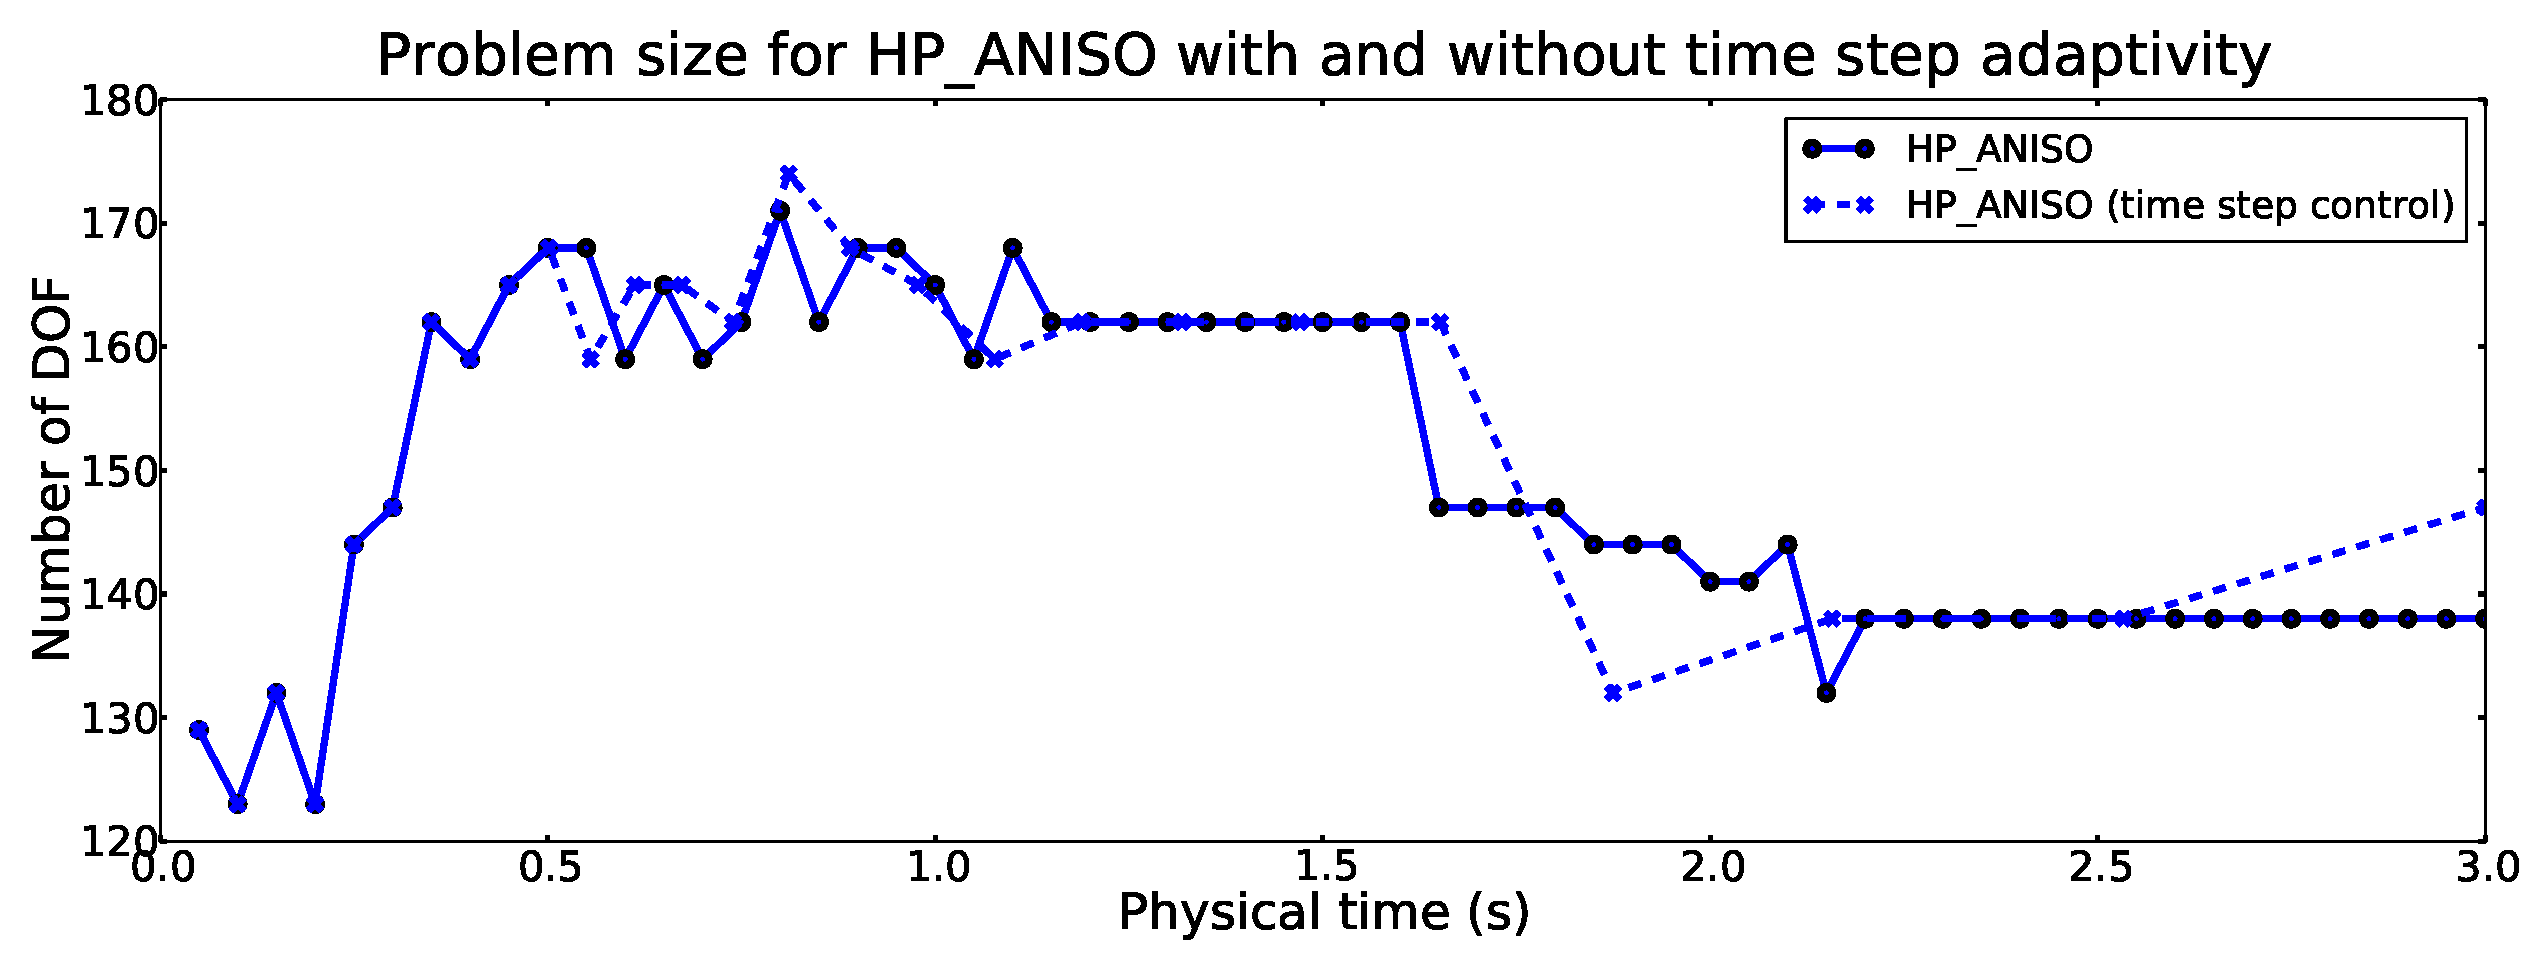
\includegraphics[width=\columnwidth]{timeadapt_dof}
  \caption{\label{fig:timeadapt_dof} Number of DOF
  as a function of physical time for HP\_ANISO with and without
  time step adaptivity. The markers on the graphs indicate the
  time steps.}
  \end{centering}
\end{figure}
\begin{figure}[!ht]
  \begin{centering}
  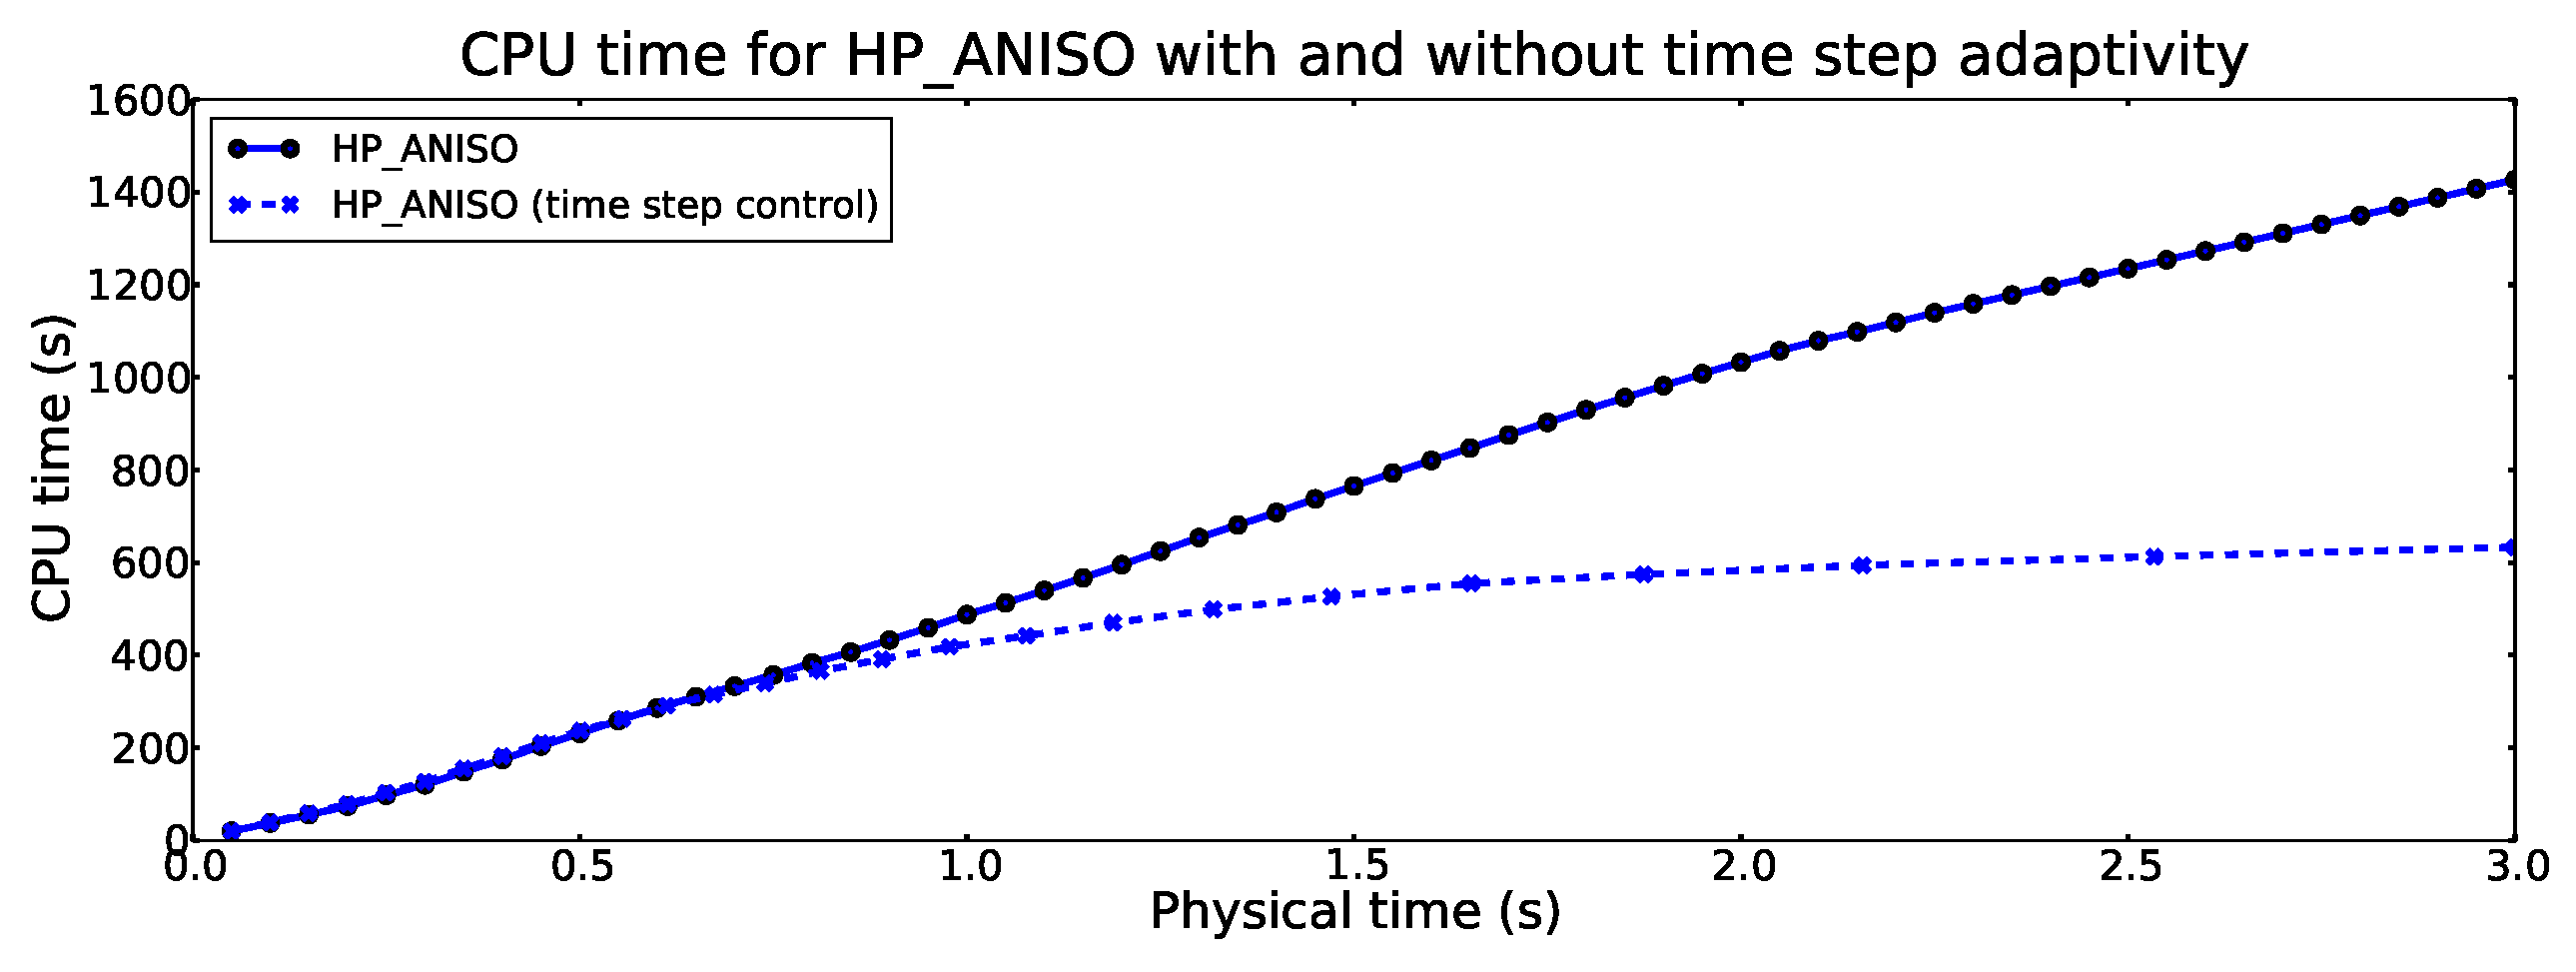
\includegraphics[width=\columnwidth]{timeadapt_cpu}
  \caption{\label{fig:timeadapt_cpu} Cumulative CPU times
  as a function of physical time for HP\_ANISO with and without
  time step adaptivity. The markers on the graphs indicate the
  time steps.}
  \end{centering}
\end{figure}

To optimize the calculation time of HP\_ANISO, an adaptive time step control was employed.
The classical PID controller was used~\cite{valli2002control,dubcova2010space}.
Since $c$ and $\varphi$ change differently in time as was demonstrated in Figs.~\ref{fig:cphi-1}
and~\ref{fig:cphi-2}, the relative changes between the solutions at different
time steps were monitored:
\begin{eqnarray}
  e_c^n & = & \frac{\lVert c^n-c^{n-1}\rVert}{\lVert c^n \rVert},\\
  e_\varphi^n & = & \frac{\lVert \varphi^n-\varphi^{n-1}\rVert}{\lVert \varphi^n \rVert}.
\end{eqnarray}
The relative changes to control the time step was calculated as follows:
\begin{equation}
  e^n=\max\left\{ e_c^n,\ e_\varphi^n \right\}.
\end{equation}
If $e^n < \delta$ where $\delta>0$ is a defined tolerance, then the time
step for the next iteration is increased smoothly to
\begin{equation}
  \delta\tau^{n+1}=\left( \frac{e^{n-1}}{e^n} \right)^{k_P}\ \left( \frac{\delta}{e^n} \right)^{k_l}\
  \left[ \frac{\left( e^{n-1} \right)^2}{e^n e^{n-2}} \right]^{k_D} \delta\tau^n,
\end{equation}
where parameters are from~\cite{valli2002control}:
\begin{equation}
  k_p=0.075,\quad k_l=0.175,\quad k_D=0.01.
\end{equation}
The tolerance $\delta$ was set to $\delta=0.25$ in the current optimization
example. At this point, the implementation does not support
adaptive time stepping if $e^n\geq \delta$. However, the implementation 
of advanced adaptive higher-order time-stepping methods is in progress.
The calculated $e_c^n$ and $e_\varphi^n$ are shown in Fig.~\ref{fig:cphirelerr}.
The HP\_ANISO problem size and computing time with and without time step control
are shown in Figs.~\ref{fig:timeadapt_dof} and~\ref{fig:timeadapt_cpu}. The reader
can notice that the computing time was reduced more than two times when the time
step control was employed.

\subsection{HP\_ANISO adaptivity with physically more realistic boundary conditions}
\begin{figure}[!ht]
  \begin{centering}
  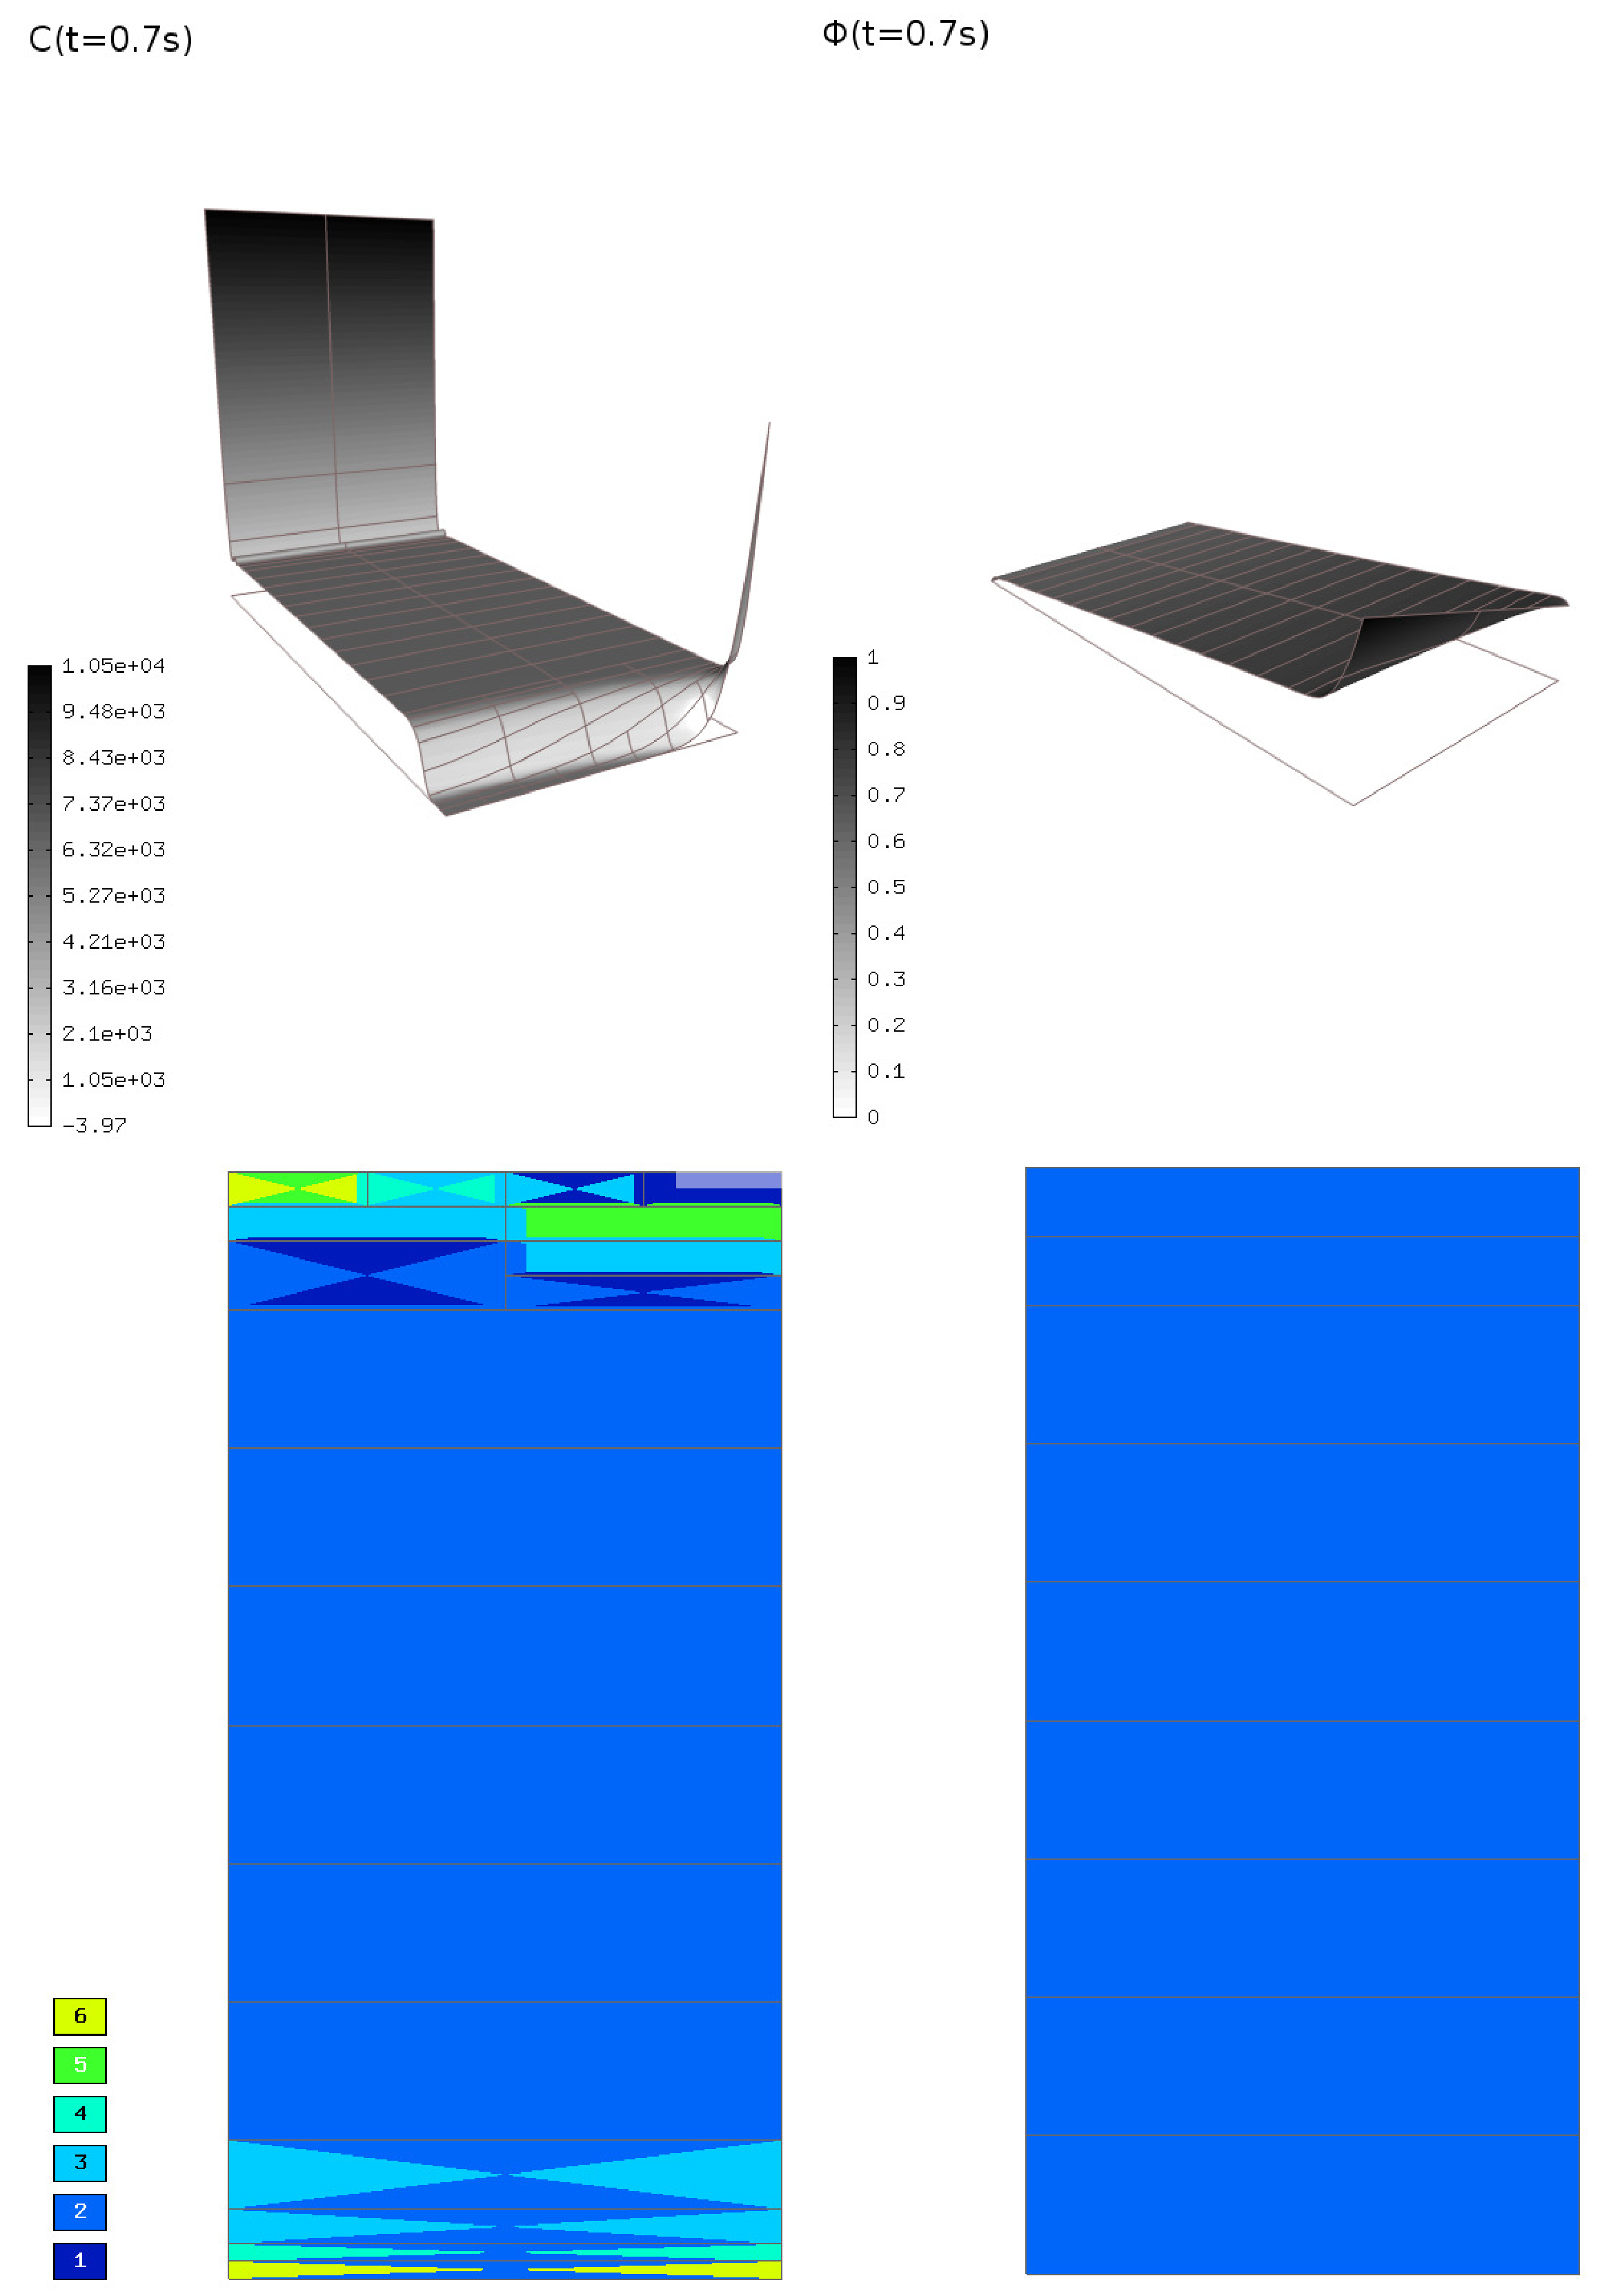
\includegraphics[width=\columnwidth]{cphiorders}
  \caption{\label{fig:cphi-orders} Solutions $c$ and $\varphi$
  and corresponding polynomial degrees of the elements at
  $t=0.1\ s$. HP\_ANISO refinement mode was used. The height
  in the solution graphs indicates the value.}
  \end{centering}
\end{figure}

In real physics calculations, the applied voltage on boundary $\partial\Omega_1$
is not constant. This can be, for instance, due to the high resistance of
the electrodes as explained in~\cite{pugal2009}.
To see how the HP\_ANISO adaptivity works for such situations, the
voltage on the boundary was applied as follows:
\begin{equation}
  \phi_{\Omega_1}\left( x \right)=0.5\left[V \right] \frac{x\left[ m \right ]}{\text{width}_{\Omega_1}\left[ m \right]}+0.5\left[ V \right],
\end{equation}
where $\text{width}_{\Omega_1}$ is the width of the boundary. The given boundary is effectively
a linear incrase of the voltage from $\phi_{\Omega_1}\left(x = 0 \right)=0.5\ V$ to
$\phi_{\Omega_1}\left(x=\text{width}_{\Omega_1}\right) = 1.0\ V$.
Now the concentration gradient $\nabla c$ and the voltage gradient $\nabla \varphi$ are no
longer effectively in 1D.

The calculated scaled values $c$ and $\varphi$ in $\Omega$ and corresponding meshes and polynomial
degrees of the elements at $t=0.1\ s$ are shown in Fig.~\ref{fig:cphi-orders}.
Notice that the solution
is different to the one in Fig.~\ref{fig:cphi-1}. The HP\_ANISO
adaptivity algorithm has particularly increased the polynomial degree
and refined the mesh near $\Omega_1$ where a sharp concentration
peak exists (compare to Fig.~\ref{fig:poly}).
At $t=3.0\ s$, the shape of the solutions $c$ and $\varphi$ are similar to the one
in Fig.~\ref{fig:cphi-2} and therefore the polynomial space and mesh gets adapted
accordingly. This example clearly illustrates how 
the solution of PNP with non-uniform
boundary conditions is very dynamic in time
and how the HP\_ANISO time dependent adaptivity 
finds an optimal mesh and polynomial space to adapt to the dynamics
of the problem. 

\subsection{Length scale analysis}

\begin{figure}[!ht]
  \begin{centering}
  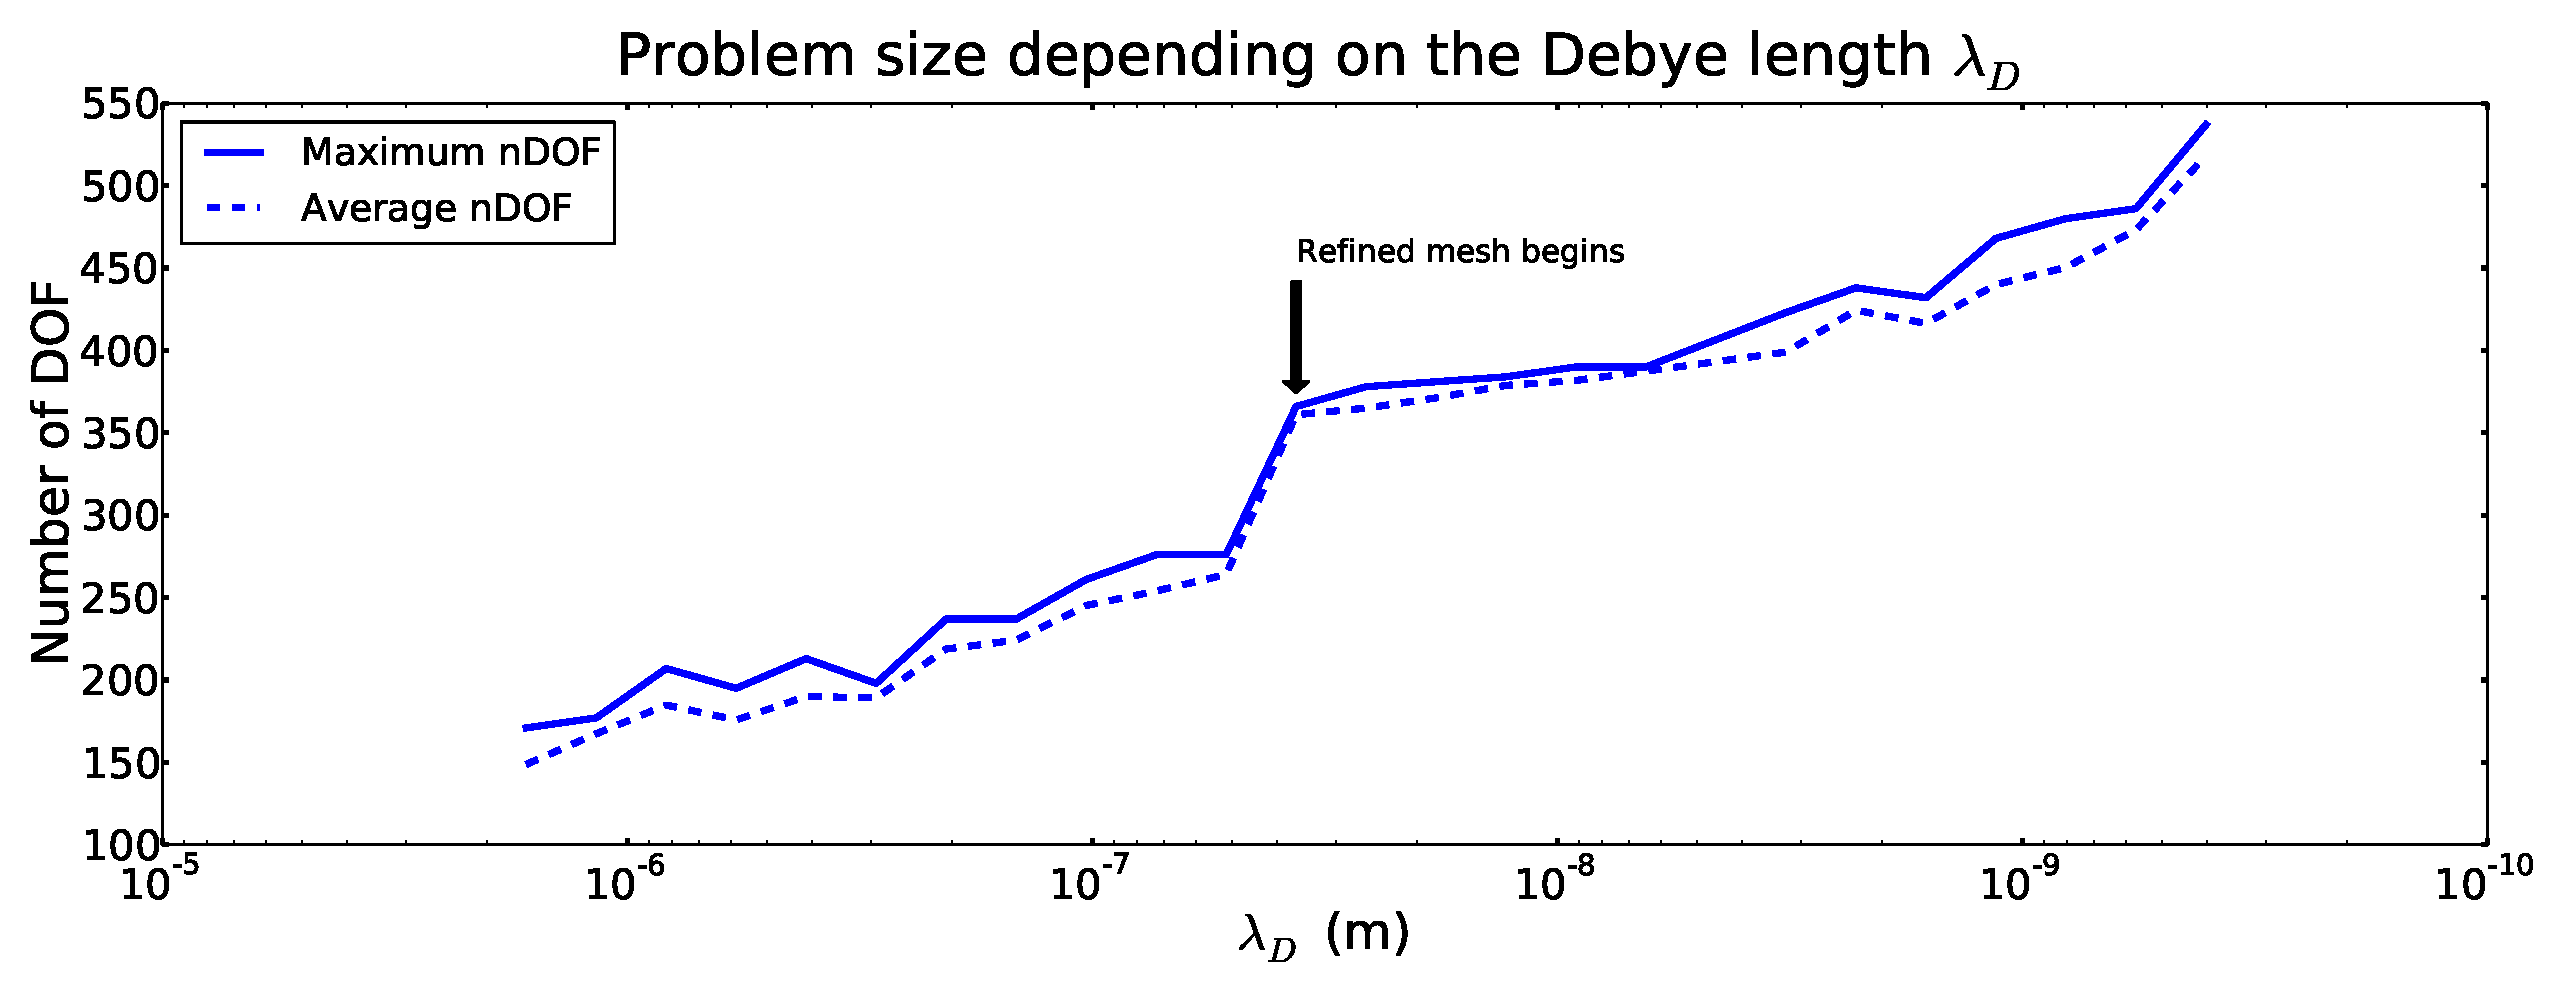
\includegraphics[width=\columnwidth]{debye_dof}
  \caption{\label{fig:debye_dof} Problem size depending on the
	Debye length. Initially the coarse mesh (shown in Fig.~\ref{fig:mesh}~(a))
	was used. It was necessary to use the fine mesh (see Fig.~\ref{fig:mesh}~(c)) 
	for smaller $\lambda_D$ values.}
  \end{centering}
\end{figure}

\begin{figure}[!ht]
  \begin{centering}
  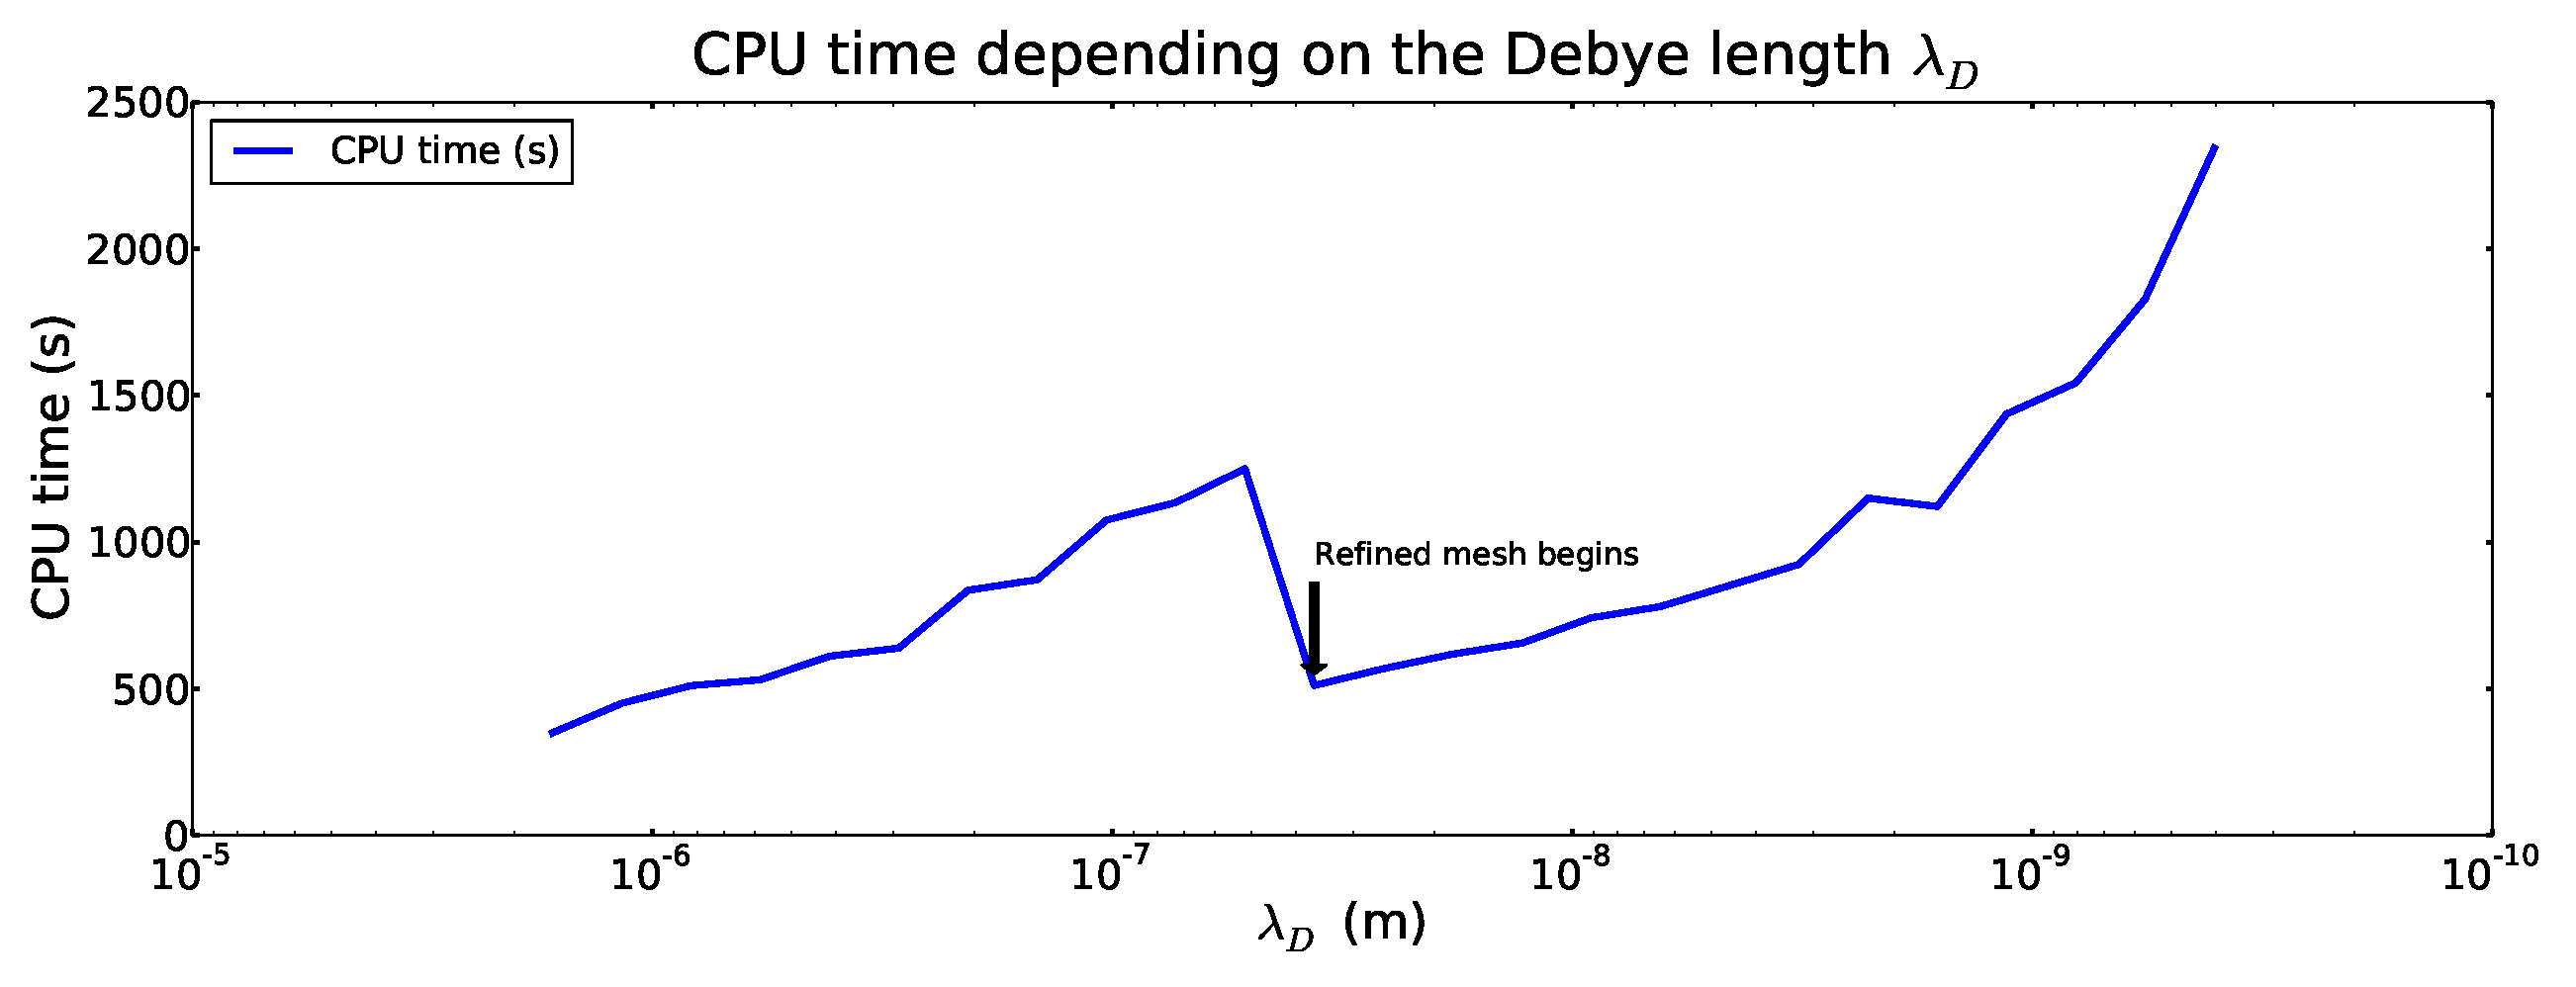
\includegraphics[width=\columnwidth]{debye_cpu}
  \caption{\label{fig:debye_cpu} CPU time depending on the
	Debye length. Initially the coarse mesh (shown in Fig.~\ref{fig:mesh}~(a))
	was used. It was necessary to use the fine mesh (see Fig.~\ref{fig:mesh}~(c)) 
	for smaller $\lambda_D$ values.}
  \end{centering}
\end{figure}
The Debye length $\lambda_D$ is the screening length in the electrolyte
solutions. Its numerical value shows the
thickness of the charged layer in the vicinity of the boundaries $\partial\Omega_1$ 
and $\partial\Omega_2$.
In all the previous simulations, the Debye screening length was determined by  the constants in
Table~\ref{Table:used-constants} and Eq.~\ref{eq:debye}: $\lambda_D=1.7\ \mu m$. It is known that computation gets increasingly
difficult when reducing the value of $\lambda_D$.
It was our interest to see how small screening lengths can Hermes HP\_ANISO automatic
adaptivity handle. The parameter $\varepsilon$ was varied as follows:
$$\varepsilon_n=\varepsilon\times 0.5^n,$$ where $\varepsilon$ is taken from Table~\ref{Table:used-constants}. The simulations were run for each $\varepsilon_n$ and corresponding $\lambda_D$ value
and maximum number of degrees of freedom and cumulative CPU time were recorded.
The simulation time $t$ for each $\lambda_D$ was chosen to be $\tau$ --- the
characteristic time scale --- and each simulation
was divided equally into fifteen time steps. The PID controller was not used.
Fig.~\ref{fig:debye_dof} shows the maximum and average number of degrees of 
freedom during calculation
as a function of the Debye length and Fig.~\ref{fig:debye_cpu} shows cumulative CPU time as a function
of the Debye length. The simulations up to $0.52\ nm$
screening length were carried out on
the initial coarse mesh. However, from $\lambda_D > 0.52\ nm$, the finer initial mesh had to
be used so the existence of the large gradients of the
physical fields $c$ and $\varphi$ near the boundaries could be captured in the first place.
\begin{figure}[!ht]
  \begin{centering}
  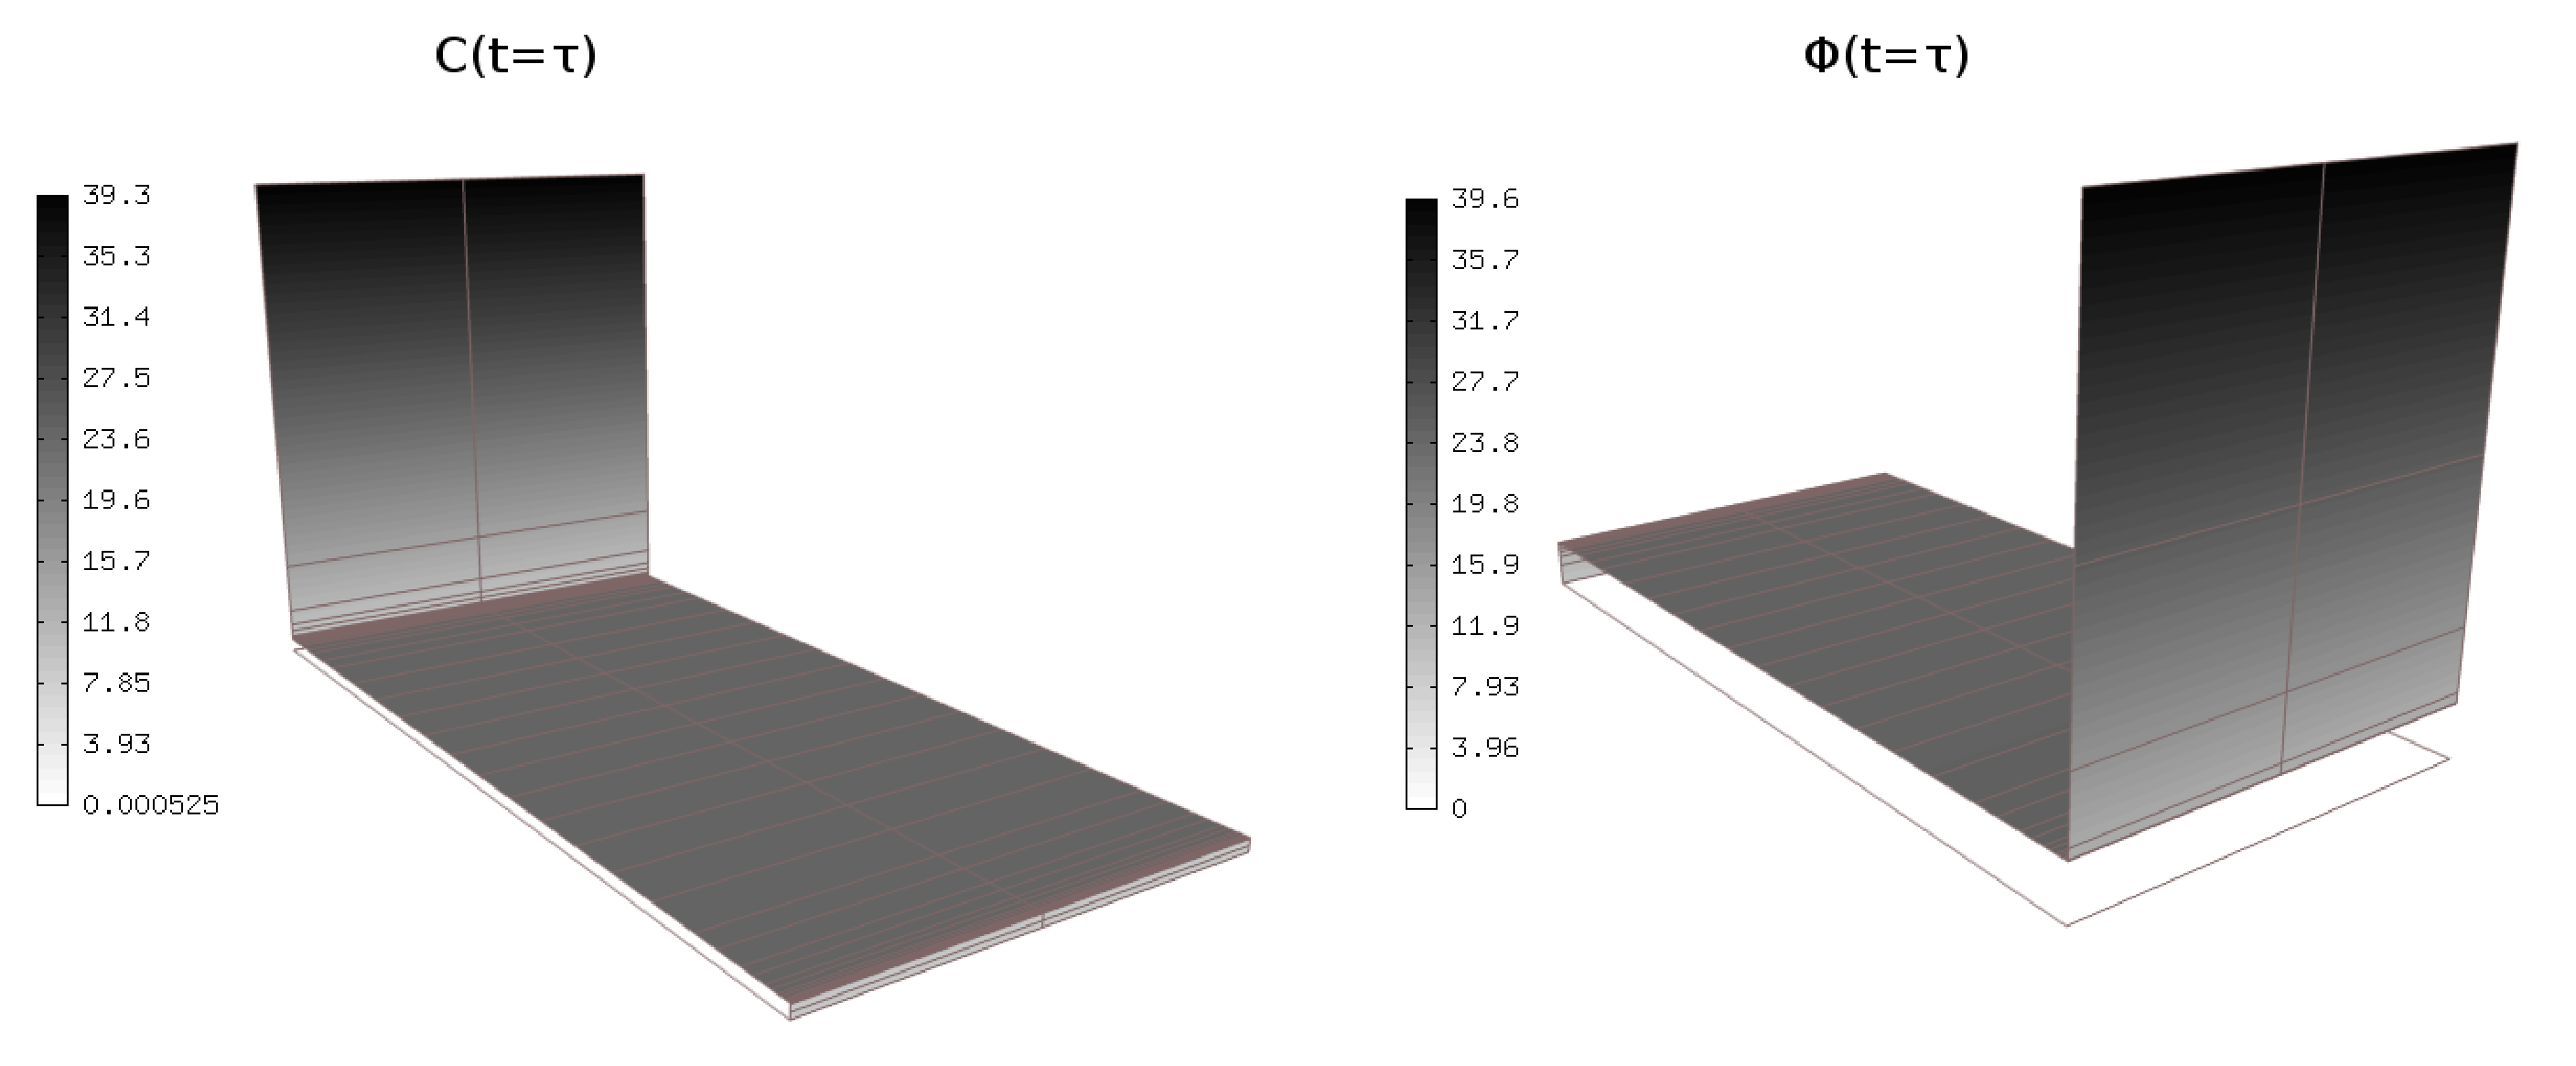
\includegraphics[width=\columnwidth]{cphitau}
  \caption{\label{fig:cphitau} Calculated fields $c$ and $\varphi$ at $t=\tau=0.81\ ms$
	for $\lambda_D=0.4\ nm$.}
  \end{centering}
\end{figure}
\noindent
The fine mesh allowed simulations with the Debye length down to $0.40\ nm$~m. The calculated
$c$ and $\varphi$ at $t=\tau$ for $\lambda_D=0.40\ nm$ are shown in Fig.~\ref{fig:cphitau}.
It appears that when using even finer initial mesh and higher initial polynomial degrees, even
smaller Debye lengths could be used when necessary. The polynomial space of $c$ had
consistently higher maximum polynomial degree than that of $\varphi$, however, the difference
was less noticeable for smaller Debye lengths.
